\chapter{Appendices for Chapter \ref{chap:mtask}}
\label{app:mtask}

\section{Data preparation}
\label{app:mtask:sec:datasets}

The general goal of the pre-processing is to obtain images which dimensions are compatible with state of the art neural networks (\eg ResNet \cite{he2016deep}, DenseNet \cite{huang2017densely}) and that are properly labeled. Classification (CLF) datasets already had classes associated to each image. For these datasets, we have thus kept the original classes. When datasets had large input images, we have further splitted them into smaller patches (see Table \ref{app:mtask:tab:details_trans_clf}).

We have considered the detection (DET) datasets to be the ones that contained several objects per input image where each object was usually denoted by a point annotation, and sometimes a label (\eg Warwick CRC \cite{sirinukunwattana2016locality}). For those datasets, the transformations were more involved (see Table \ref{app:mtask:tab:details_trans_det}). When the concentration of annotations was high (\ie a typical patch in the image contains tens of annotations) and/or the input image size was small (\ie $<$ 1k pixels square), overlapping patches were extracted. Each patch was associated a binary class indicating whether the entity to detect was present or absent in this patch. When a label was available, the associated class was chosen to indicate the presence of one type of object versus the other(s). For datasets where the objects to detect were fewer and more scattered over the input images (\eg mitosis detection), the previous approach was inappropriate as it would have yielded highly imbalanced datasets. Therefore, in this case, negative patches were still sampled exhaustively with an overlap but positive patches were sampled around the objects of interest with random shifts, yielding several samples per object. 

For the segmentation (SEG) datasets (see Table \ref{app:mtask:tab:details_trans_seg}), the patch sampling was the same as for the detection (\ie exhaustive with overlap). The class was determined if the surface ratio of the positive entity (\eg tumor) in the patch exceeded a threshold (\eg 10\% of the patch). The only exception is \textit{Breast1} dataset for which the class of the patch is the class of its central pixel. Camelyon16 \cite{bejnordi2017diagnostic} dataset was applied an additionnal pre-processing to exclude most of the whole-slide image (WSI) background.

The last transformation step was to split each resulting dataset into some training, validation and test sets for future training. We have followed a rigorous splitting process: whenever possible we have made sure that images from a same patient, or a same slide were not in two different sets. Sometimes, none of those information were available in which case we have randomly split the data. Moreover, we have ensured that all classes were present in all sets.

Resulting classification datasets and their splits are listed in Table \ref{app:mtask:tab:final_datasets}. Selected samples for each of our final classification tasks are given in Figure \ref{fig:mtask:dataset_samples}.

\begin{table}
  \centering
  \tiny
  \begin{tabular}{|c|c|c|}
  \hline
  Dataset & Patches \\
  \hline
  BACH1018 Micro & 512 $\times$ 512 \\
  Stroma LBP & original \\
  UMCM Colorectal & original \\
  Janowczyk & original \\ 
  Janowczyk & 384 $\times$ 384 \\
  \hline
  \end{tabular}
  \caption{Details for classification datasets transforms. Patches indicate whether the final patches are the \textit{original} images. Provided dimensions indicate that patches of those dimensions were extracted from the original images to make the final classification datasets.}
  \label{app:mtask:tab:details_trans_clf}
\end{table}

\begin{table}[t]
  \centering
  \scriptsize
  \begin{tabular}{|c|c|c|c|c|}
  \hline
  Dataset & Positive & Negative & Other & Dim. / Sup. \\
  \hline
  Warwick CRC & {$\left\{\text{Inflammatory}\right\}$} & {$\left\{\text{Epithelial}, \text{Fibroblast},\right.$} & / & 100 $\times$ 100 / none \\
  & & {$\left.\text{Others}, \emptyset\right\}$} & & \\
  TUPAC2016 Mitosis & {$\left\{\text{Mitosis}\right\}$} & {$\left\{\emptyset\right\}$} & / & 250 $\times$ 250 / 10 \\
  MITOS-ATYPIA & {$\left\{\text{Mitosis}\right\}$} & {$\left\{\emptyset\right\}$} & {$\left\{\text{NonMitosis}\right\}$} & 323 $\times$ 323 / 10 \\
  Janowczyk 5 & {$\left\{\text{Mitosis}\right\}$} & {$\left\{\emptyset\right\}$} & / & 250 $\times$ 250 / 10 \\
  \hline
  \end{tabular}
  \caption{Details for detection datasets transforms. Columns \textit{Positive} and \textit{Negative} indicate which annotation information or label was used to set respectively the patch class as positive or negative. The $\emptyset$ means "\textit{no annotation}". \textit{Dim} and \textit{Sup} stand for \textit{Dimensions} and \textit{Supersample}. The former indicates whether or not the positive patches was supersampled, and if so, how many patches were extracted per positive annotation.}
  \label{app:mtask:tab:details_trans_det}
\end{table}

\begin{table}[t]
  \centering
  \scriptsize
  \begin{tabular}{|c|c|c|c|c|c|c|c|c|c|c|}
  \hline
  \multirow{2}{*}{Dataset} & \multicolumn{3}{c}{Classes} & \multicolumn{3}{|c|}{Dimensions} & \multirow{2}{*}{WSI} & \multirow{2}{*}{P/CW} \\
  \cline{2-7}
  & Positive & Negative & Area {\small($\%$)} & Extracted & Rescaled & Overlap & & \\
  \hline
  Janowczyk 1 & {$\left\{\text{Nuclei}\right\}$} &  {$\left\{\emptyset\right\}$} & 5 & 250 $\times$ 250 & / & 125 & no & / \\
  Janowczyk 2 & {$\left\{\text{Epithelium}\right\}$} &  {$\left\{\emptyset\right\}$} & 10 & 200 $\times$ 200 & / & 100 & no & / \\
  Camelyon 16 & {$\left\{\text{Tumor}\right\}$} &  {$\left\{\emptyset\right\}$} & 10 & 768 $\times$ 768 & 384 $\times$ 384 & 0 & yes & 1000 \\
  Breast1 & {$\left\{\text{InSitu, Infiltration}\right\}$} & {$\left\{\emptyset\right\}$} & / & 384 $\times$ 384 & / & / & no & /\\
  Breast2 & {$\left\{\text{InSitu, Infiltration}\right\}$} & {$\left\{\emptyset\right\}$} & 10 & 250 $\times$ 250 & / & 125 & no & /\\
  \hline
  \end{tabular}
  \caption{Details for segmentation datasets transforms. \textit{Area} is the surface threshold we have used to separate positive from negative patches (if surface of positive annotation was larger than the given value, then the patch was considered positive). Column "\textit{WSI}" indicates that the original images are whole-slide images and were applied additional pre-processing to remove background tiles. Column "\textit{P/CW}" indicates whether or not the patches were subsampled. If a value is provided, this value is the maximum number of samples per class per WSI capped that was produced.}
  \label{app:mtask:tab:details_trans_seg}
\end{table}

\begin{table}[t]
  \centering
  \scriptsize
    \begin{tabular}{|c|c|r:r|r:r|r:r|r:r|c|}
\hline
\multirow{2}{*}{\textbf{Name}} & \multirow{2}{*}{\textbf{Cls}} & \multicolumn{2}{c|}{\textbf{Train}} & \multicolumn{2}{c|}{\textbf{Val}} & \multicolumn{2}{c|}{\textbf{Test}} & \multicolumn{2}{c|}{\textbf{Total}} & \multirow{2}{*}{\textbf{Split}} \\
\cline{3-10}
 & &  \multicolumn{1}{c:}{\textbf{Img.}} & \multicolumn{1}{c|}{\textbf{p/s}} & \multicolumn{1}{c:}{\textbf{Img.}} & \multicolumn{1}{c|}{\textbf{p/s}} & \multicolumn{1}{c:}{\textbf{Img.}} & \multicolumn{1}{c|}{\textbf{p/s}} & \multicolumn{1}{c:}{\textbf{Img.}} & \multicolumn{1}{c|}{\textbf{p/s}} & \\
\hline
Necrosis & 2 & 695 & 9 & 96 & 1 & 91 & 3 & 882 & 13 & slide \\
ProliferativePattern & 2 & 1179 & 19 & 167 & 4 & 511 & 13 & 1857 & 36 & slide \\
CellInclusion & 2 & 1643 & 21 & 173 & 2 & 1821 & 22 & 3637 & 45 & slide \\
MouseLba & 8 & 1722 & 9 & 716 & 4 & 1846 & 7 & 4284 & 20 & slide \\
HumanLba  & 9 & 4051 & 50 & 346 & 5 & 1023 & 9 & 5420 & 64 & slide \\
Lung & 10 & 4881 & 669 & 562 & 73 & 888 & 139 & 6331 & 881 & slide \\
Glomeruli  & 2 & 12157 & 10 & 2448 & 8 & 14608 & 102 & 29213 & 120 & slide \\
Breast1 & 2 & 14055 & 22 & 4206 & 8 & 4771 & 4 & 23032 & 34 & patient \\
Breast2 & 2 & 11483 & 22 & 3470 & 8 & 2570 & 4 & 17523 & 34 & patient \\
BoneMarrow & 8 & 522 & 522 & 130 & 130 & 639 & 639 & 1291 & 1291 & slide \\
Janowczyk 1 & 2 & 17550 & 77 & 4500 & 19 & 9675 & 41 & 31725 & 137 & patient \\
Janowczyk 2 & 2 & 1701 & 21 & 405 & 5 & 1296 & 16 & 3402 & 42 & patient \\
Janowczyk 5 & 2 & 16560 & 7 & 4551 & 2 & 3759 & 3 & 24870 & 12 & patient \\
Janowczyk 6 & 2 & 224822 & 230 & 31934 & 29 & 20768 & 20 & 277524 & 279 & patient \\
Janowczyk 7 & 3 & 1350 & 225 & 456 & 76 & 438 & 73 & 2244 & 374 & patient \\
MITOS-ATYPIA & 3 & 40364 & 13 & 12799 & 4 & 11710 & 5 & 64873 & 22 & slide \\
Warwick CRC & 2 & 1500 & 60 & 500 & 20 & 500 & 20 & 2500 & 100 & image \\
Camelyon 16 & 2 & 237753 & 221 & 27950 & 26 & 26523 & 24 & 292226 & 271 & slide\\
TUPAC2016 Mitosis & 2 & 62874 & 526 & 7827 & 74 & 7152 & 56 & 77853 & 656 & patient \\
Stroma LBP & 2 & 947 & 492 & 407 & 228 & 959 & 656 & 2313 & 1376 & image \\
BACH2018 Micro & 4 & 2760 & 143 & 720 & 52 & 1320 & 89 & 4800 & 284 & patient \\
UMCM Colorectal & 8 & 3349 & 6 & / & / & 1651 & 4 & 5000 & 10 & patient \\
\hline
\textbf{Total} & 81 & 663918 & 3374 & 104363 & 778 & 114519 & 1949 & 882800 & 6101 & / \\
\hline
    \end{tabular}
    
    \caption{Classification datasets generated from the collected datasets. \textit{p/s} indicate the number of distinct patients, or slides (if no patient information was available), or images (in case when none of the two information were available) in the set. The column \textit{Split} indicates whether the dataset was split patient, slide or image-wise.}
    \label{app:mtask:tab:final_datasets}
\end{table}

\section{A note about batch normalization}
\label{app:mtask:sec:batch_norm}

It has been shown that a network equipped with batch normalization \cite{ioffe2015batch} can exhibit issues when it is used across different domains \cite{li2018adaptive, chang2019domain}. A similar issue occurs when transferring such network to one (or several) target task of which the input distribution(s) differ(s) greatly from the source task. Indeed, the first iteration will propagate through the network samples from an unseen and likely different distribution which will trigger a massive change of batch normalization module statistics ($\mu_\mathcal{B}$ and $\sigma_\mathcal{B}$). However, the batch normalization trainable parameters ($\beta$ and $\gamma$) will themselves be updated much more slowly (especially when the training learning rate is small) preventing them to adapt properly to the shift in distribution and statistics. In the context of this work, early experiments have shown that it had a undesirable negative effect on training basically destroying the purpose of transfer, as the training curves exhibited a similar behavior to training from scratch. This problem was aggravated in multi-task learning when several tasks, with different input distributions, were used. We have applied a simple procedure to attenuate this effect. Our idea consists in updating parameters $\beta$ and $\gamma$ of each batch normalization module before starting training such that the output of the module is preserved when the shift in distribution occurs. Given a source task $\mathcal{D}_s$ and a target task $\mathcal{D}_t$, few batches of the target task are forwarded into the network to estimate the new statistics $\mu_{\mathcal{B}_t}$ and $\sigma_{\mathcal{B}_t}$ of each batch normalization module input. Based on the obtained statistics, the new parameters $\beta_s$ and $\gamma_s$ for a module are given by (see below for the derivation of these formulas):
\begin{eqnarray}
\gamma_t &=& \gamma_s \dfrac{\sigma^{(\epsilon)}_{\mathcal{B}_t}}{\sigma^{(\epsilon)}_{\mathcal{B}_s}}\label{app:mtask:eqn:bn_update_gamma}\\
\beta_t &=& \beta_s + \gamma_s  \dfrac{(\mu_{\mathcal{B}_t}-\mu_{\mathcal{B}_s})}{\sigma^{(\epsilon)}_{\mathcal{B}_s}}\label{app:mtask:eqn:bn_update_beta}
\end{eqnarray}
where $\mu_{\mathcal{B}_s}$, $\sigma^{(\epsilon)}_{\mathcal{B}_s}$, $\beta_s$ and $\gamma_s$ are the original source task's statistics and parameters. The expression $\sigma^{(\epsilon)}_{\mathcal{B}_x}$ denotes an altered version of standard deviation presented in the original paper which is given by $\sqrt{\sigma_{\mathcal{B}_x}^2 + \epsilon}$ with a $\epsilon$ constant added for numerical stability. In our multi-task setting, we have used batches containing samples from all tasks during the new statistics estimation in order to mimic the actual inputs distributions at training time.

\subsection*{Deriving the formulas}
A batch normalization module being a composition of linear functions, it is therefore linear and can be re-expressed as:
\begin{equation} \label{app:mtask:eqn:batch_norm_is_linear}
y_k = BN_k(x) = m_k x + p_k
\end{equation}
where $y_k$ and $x$ respectively denote the output of the batch normalization module for task $k$ (\ie using task $k$ statistics and parameters) and the input of the batch normalization module. Using the definition of the module, Equation \ref{app:mtask:eqn:batch_norm_is_linear} can be rewritten as:
\begin{equation} \label{app:mtask:eqn:batch_norm_is_linear_rewritten}
y_k = \underbrace{\dfrac{\gamma_k}{\sigma^{(\epsilon)}_{\mathcal{B}_k}}}_{m_k} x + \underbrace{\beta_k - \gamma_k\ \dfrac{\mu_{\mathcal{B}_k}}{\sigma^{(\epsilon)}_{\mathcal{B}_k}}}_{p_k}.
\end{equation}
The formula in Equations \ref{app:mtask:eqn:bn_update_gamma} and \ref{app:mtask:eqn:bn_update_beta} are obtained by ensuring $y_t = y_s$ for any $x$, or similarly solving the following system:
\begin{align}
\begin{cases}
m_s = m_t\\
p_s = p_t\\
\end{cases}
\end{align}

\section{A note about gradients}
\label{app:mtask:sec:gradients}

Because samples are routed through their respective task head in our architecture, all parts of the network do not see the same number of samples from a batch which causes the gradients to be underestimated in the network heads. This can be shown by developing the derivative of our loss with respect to one of the logits of a head. Let $r^{(i)}_{k}$ be the class $k$ logit of task $t_i$. The derivatives of the loss ${\cal L}$ (Equation 1, in the original publication) with respect to $r^{(i)}_k$ is given by:
\begin{equation} 
    \label{app:mtask:eqn:rescale_grad}
    \frac{\partial \mathcal{L}}{\partial r^{(i)}_{k}} = - \frac{1}{B} \sum_{j=1}^{\left|\mathcal{B}_{t_i}\right|} \frac{\partial \ell^{(i)}_j}{\partial r^{(i)}_{k}},
\end{equation}
where $\ell^{(i)}_j$ is the loss term for the $j$th sample of task $t_i$ in the batch sample. Equation \ref{app:mtask:eqn:rescale_grad} shows that the gradients are divided by the batch size although they are estimated using $\left|\mathcal{B}_{t_i}\right|$ samples (\ie the number of samples from task $t_i$ in the batch). This applies also to the gradients used for updating the parameters $\theta_i$ of the head. Given a task $t_i$, this magnitude reduction has the same effect as dividing the learning rate for head $\theta_i$ by a variable factor that depends on the number of samples of task $t_i$ that are present in the batch. If tasks are sampled uniformly to create a batch, one can expect this factor to be equal to the number of tasks $T$ on average. In order to avoid this phenomenon, we applied a simple trick that consists in re-scaling the gradients of each head $\theta_i$ by multiplying them by $\phi_{t_i}$:
\begin{equation}
\phi_{t_i} = \frac{B}{\left|\mathcal{B}_{t_i}\right|}.
\end{equation}
%% Equation \ref{app:mtask:eqn:rescale_grad} can be derived by developing the derivative of the loss by the logits of one head:

%% \begin{align}
%%     \frac{\partial \mathcal{T}}{\partial r^{(i)}_{k}} &= \frac{\partial}{\partial r^{(i)}_{k}} \left[- \frac{1}{B} \sum_{m=1}^T \sum_{j=1}^{\left|\mathcal{B}_{t_m}\right|} \ell^{(m)}_j \right] \\
%%     &= - \frac{1}{B} \sum_{j=1}^{\left|\mathcal{B}_{t_i}\right|} \frac{\partial \ell^{(i)}_j}{\partial r^{(i)}_{k}} \\
%% \end{align}

% \[
%   \frac{B}{\left|\mathcal{B}_{t_i}\right|} \frac{\partial \mathcal{T}}{\partial r^{(i)}_{k}} = -  \frac{1}{\left|\mathcal{B}_{t_i}\right|} \sum_{j=1}^{\left|\mathcal{B}_{t_i}\right|} \frac{\partial \ell^{(i)}_j}{\partial r^{(i)}_{k}} 
% \]

\section{Transfer performances}
\label{app:mtask:sec:transfer_perf}

Figures \ref{app:mtask:fig:bar_lrhm_densenet} and \ref{app:mtask:fig:bar_lrhm_resnet} give the transfer performance of different combination of training hyperparameters.




% \section{Acknowledgments}

% We thank our collaborators for bringing images and annotations. 

% \begin{itemize}
%  \item \textit{CellInclusion and ProliferativePatterns}: Caroline Degand and Isabelle Salmon (Erasme Hospital, Universit\'e Libre de Bruxelles)
%  \item \textit{Breast}: Michel Reginster and Philippe Delvenne (University Hospital, Li\`ege) 
%  \item \textit{Necrosis}: Natacha Leroi and Philippe Martinive (GIGA-Cancer, ULiege)
%  \item \textit{HumanLba}: Sandrine Rorive and Isabelle Salmon (Erasme Hospital, Universit\'e Libre de Bruxelles) 
%  \item \textit{MouseLba}: Natacha Rocks, Christine Fink, Fabienne Perin, and Didier Cataldo (GIGA-Cancer, ULiege) 
%  \item \textit{Lung}: 
% Natacha Rocks, Christine Fink, Fabienne Perin, and Didier Cataldo (GIGA-Cancer, ULiege) 
%  \item \textit{Glomeruli}: Vannary Meas-Yedid and Jean-Christophe Olivo-Marin (Pasteur Institute Paris), and Eric Thervet (Georges Pompidou European Hospital Paris)
% \end{itemize}



\begin{figure*}[h]
  \centering
  \begin{subfigure}{0.48\textwidth}
    \centering
    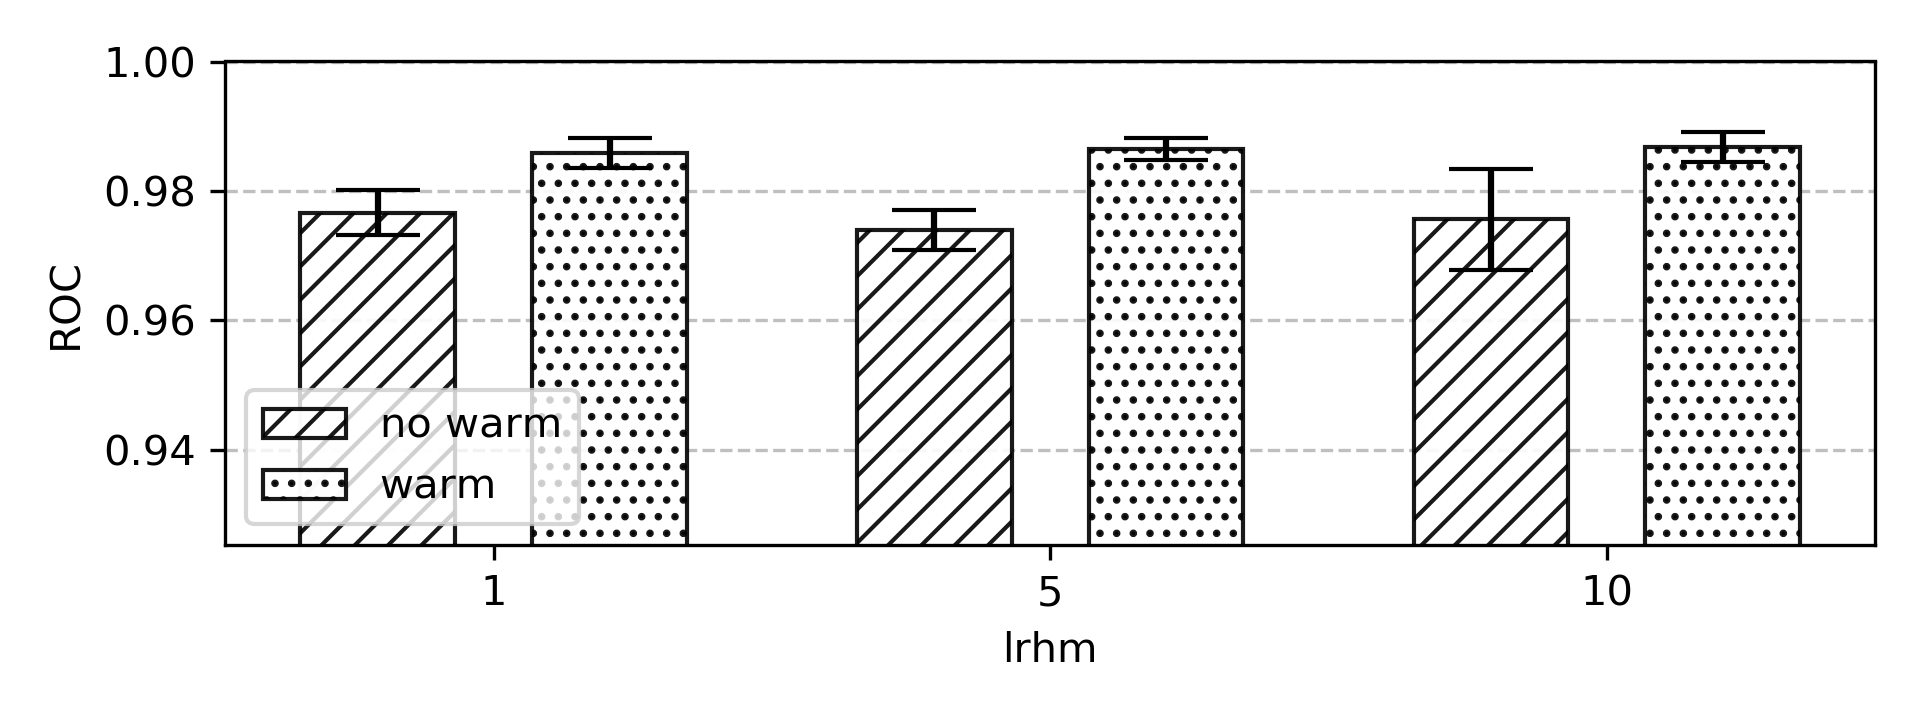
\includegraphics[width=\textwidth]{mtask/supp/bar_lrhm_1e-4_densenet121_cells_no_aug.png}
    \caption{CellInclusion}
  \end{subfigure}
  \begin{subfigure}{0.48\textwidth}
    \centering
    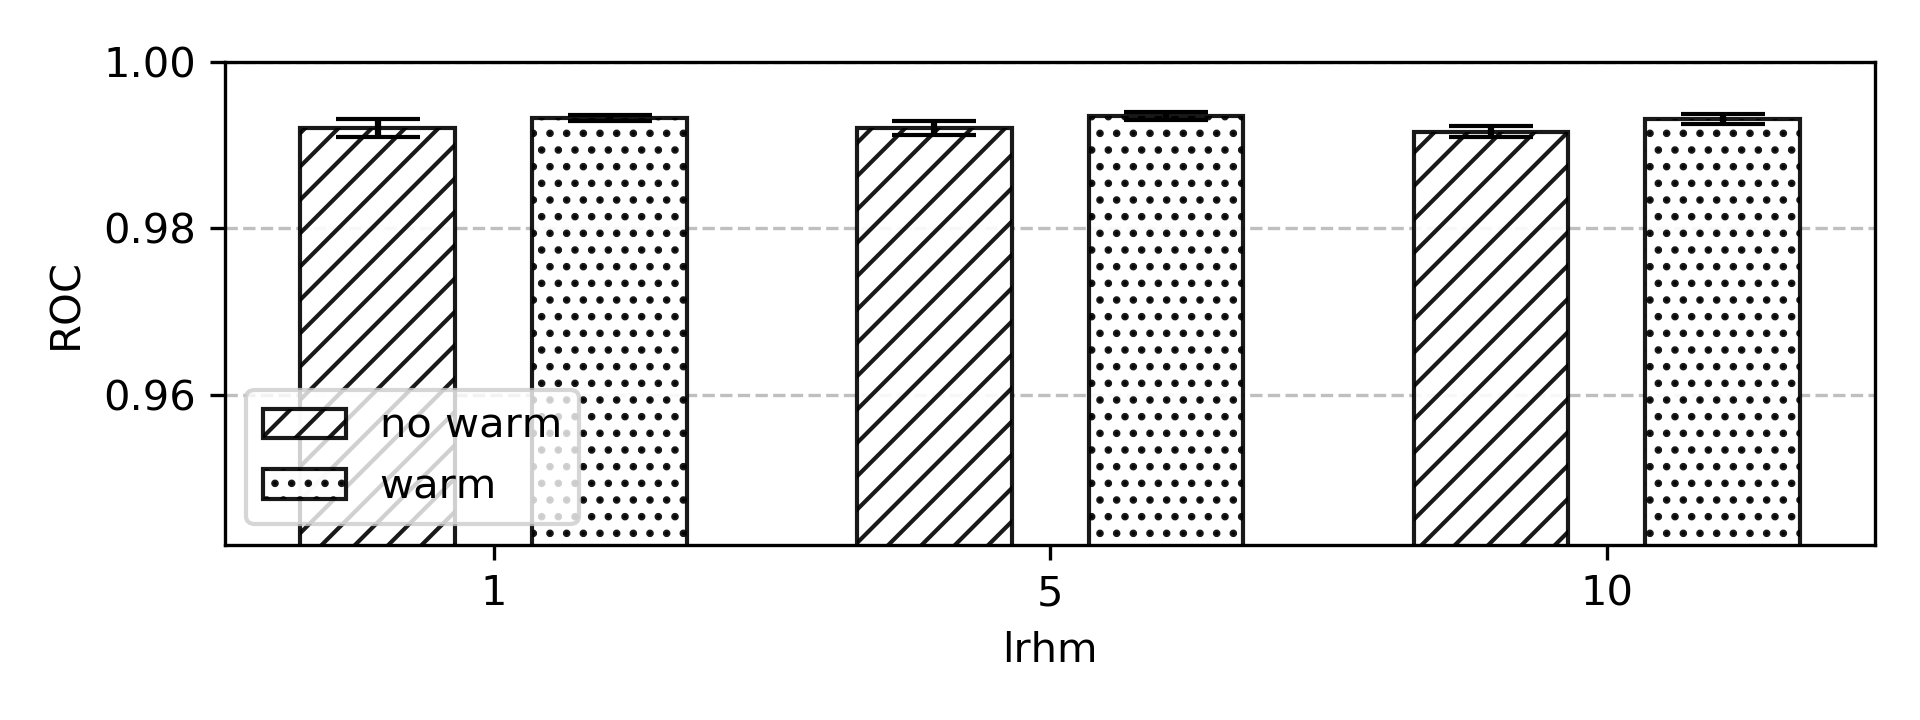
\includegraphics[width=\textwidth]{mtask/supp/bar_lrhm_1e-4_densenet121_glomeruli_no_aug.png}\\
    \caption{Glomeruli}
  \end{subfigure}
  \begin{subfigure}{0.48\textwidth}
    \centering
    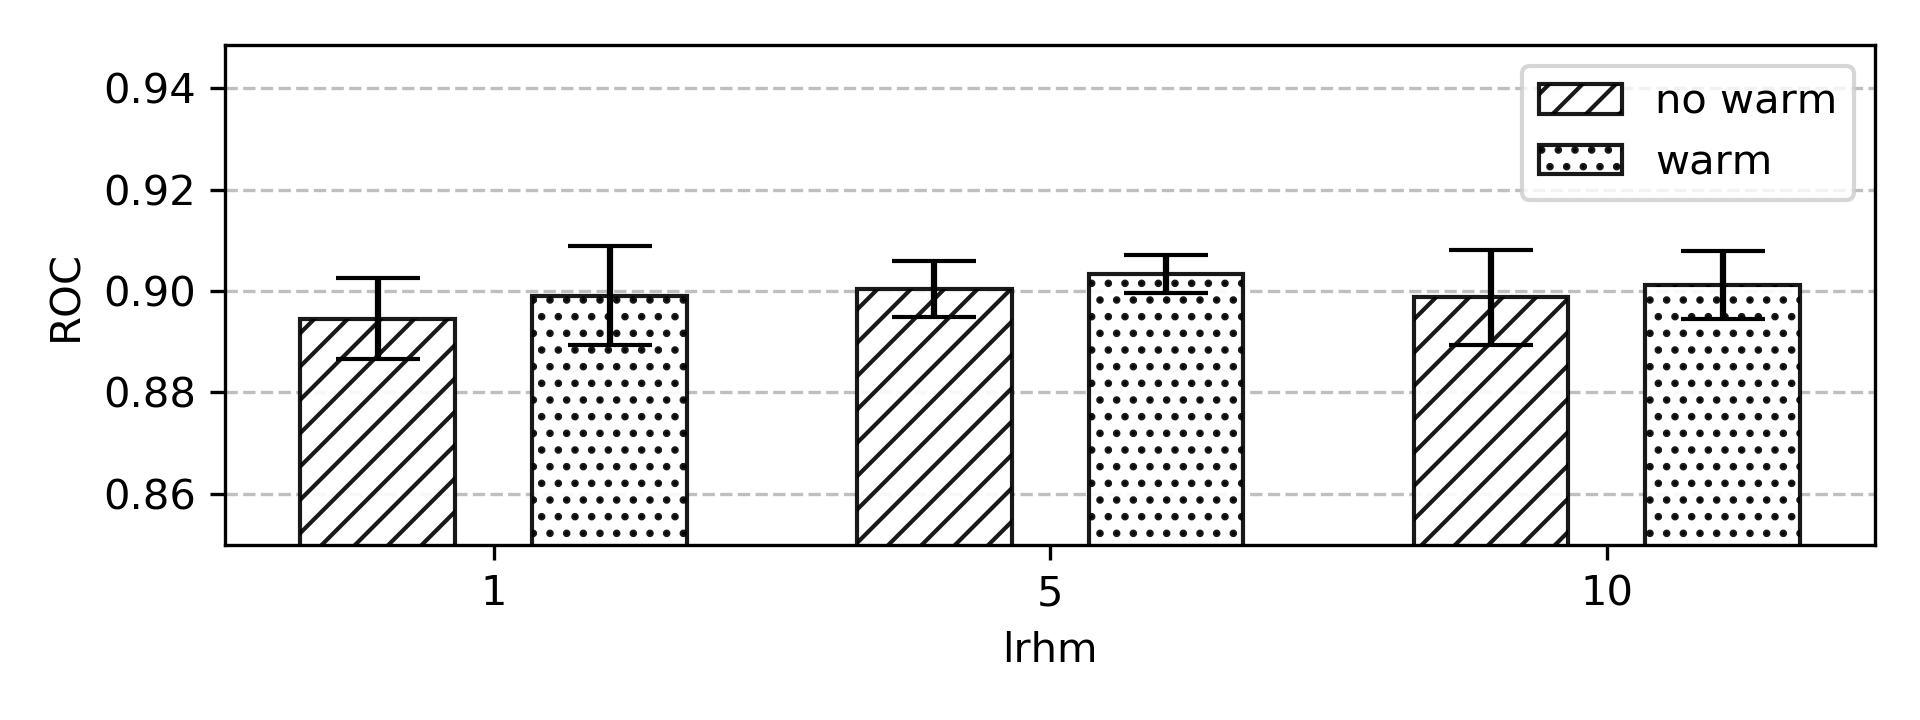
\includegraphics[width=\textwidth]{mtask/supp/bar_lrhm_1e-4_densenet121_patterns_no_aug.png}
    \caption{ProliferativePattern}
  \end{subfigure}
  \begin{subfigure}{0.48\textwidth}
    \centering
    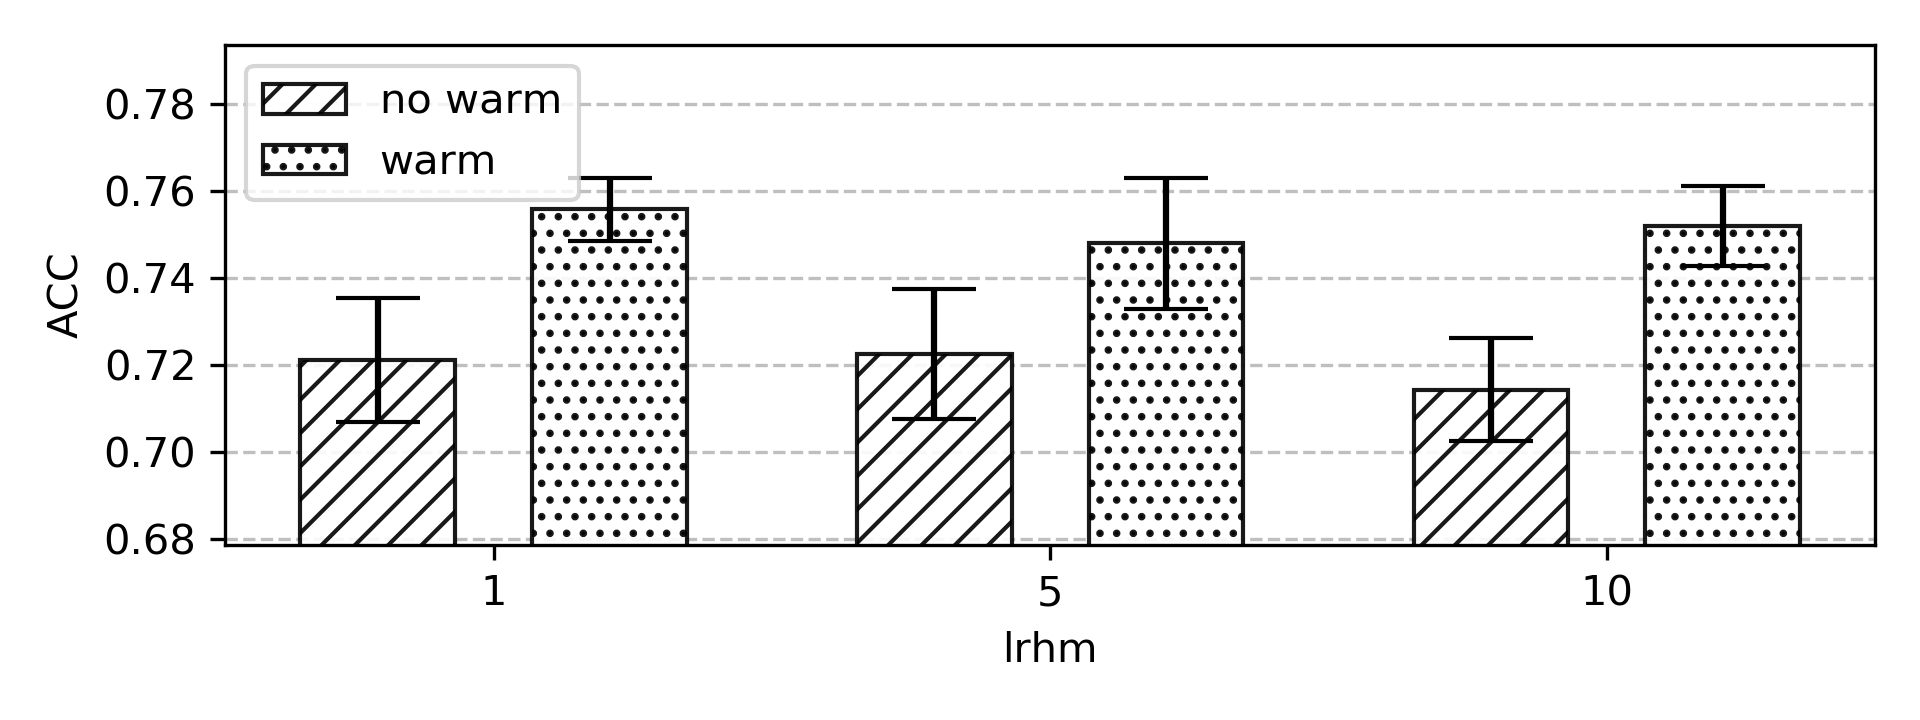
\includegraphics[width=\textwidth]{mtask/supp/bar_lrhm_1e-4_densenet121_ulb_anapath_lba.png}\\
    \caption{HumanLba}
  \end{subfigure}
  \begin{subfigure}{0.48\textwidth}
    \centering
    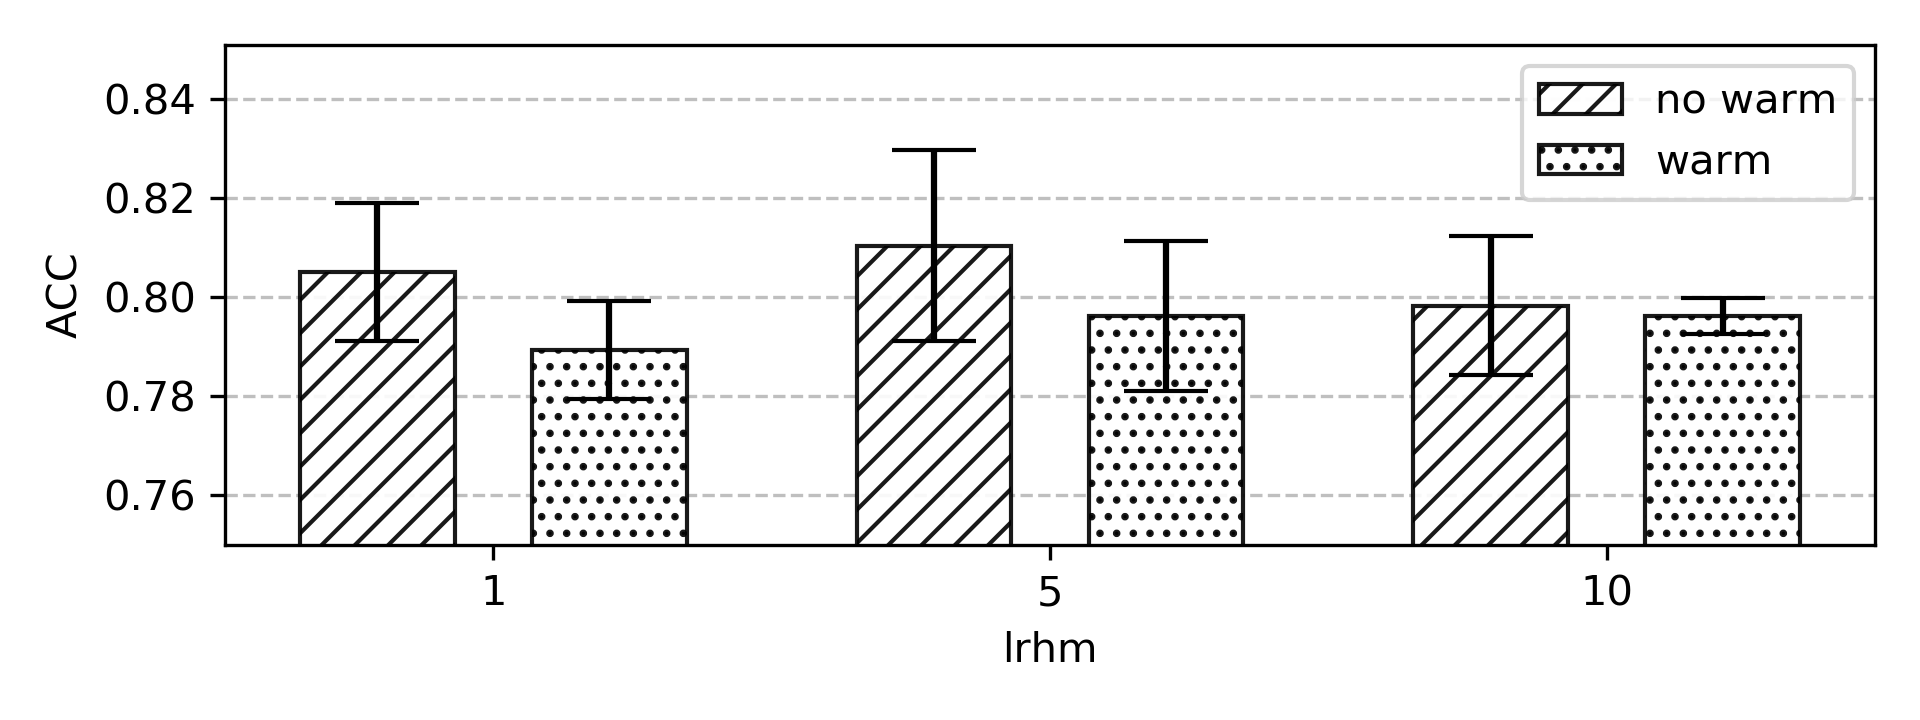
\includegraphics[width=\textwidth]{mtask/supp/bar_lrhm_1e-4_densenet121_ulg_bonemarrow.png}
    \caption{BoneMarrow}
  \end{subfigure}
  \begin{subfigure}{0.48\textwidth}
    \centering
    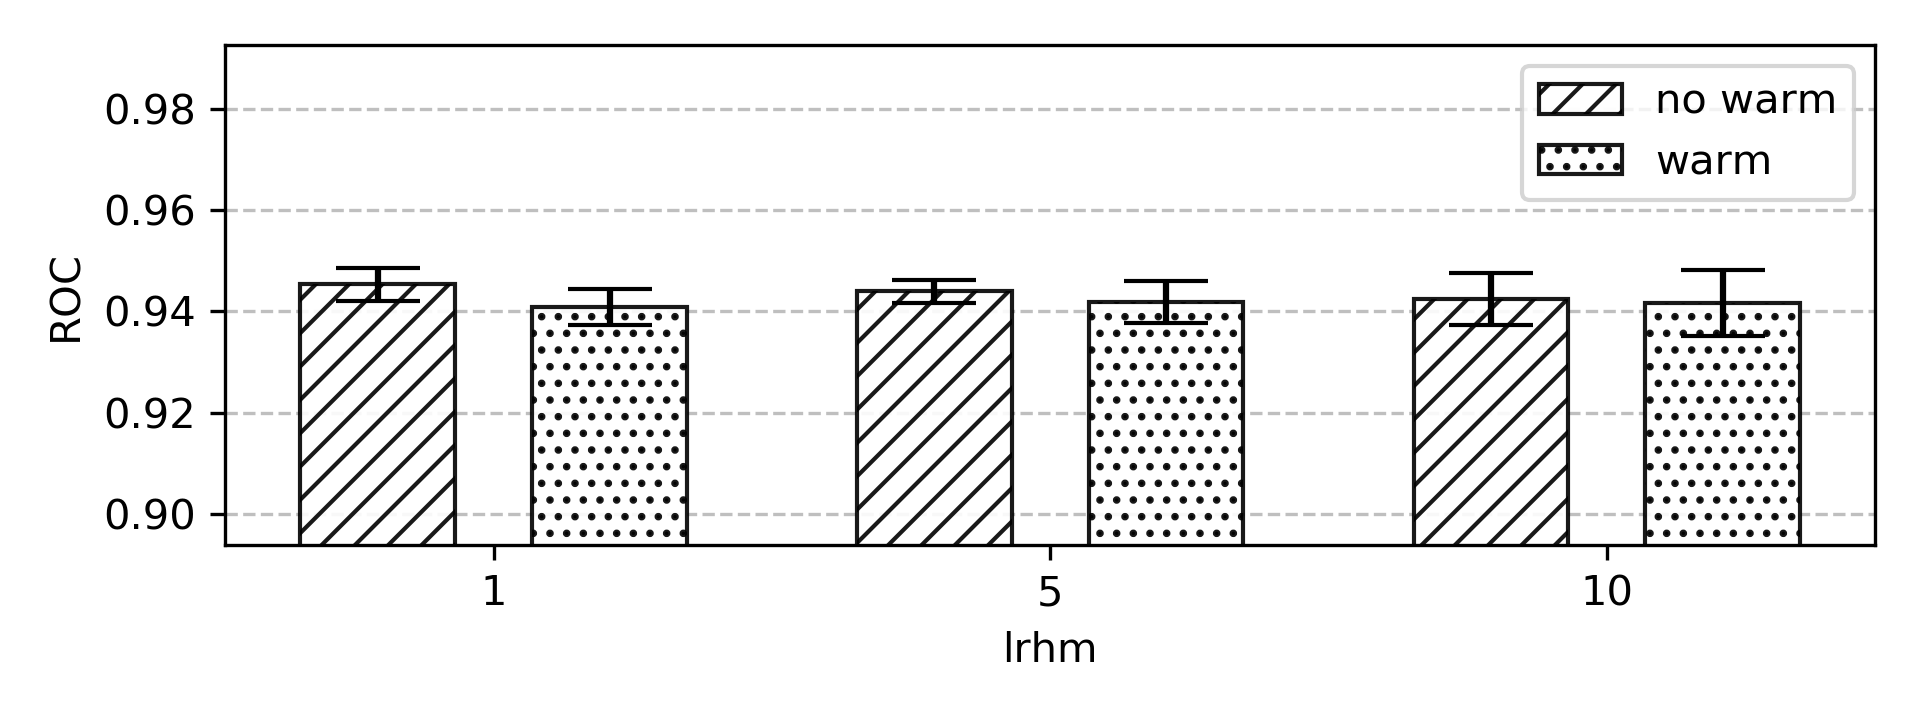
\includegraphics[width=\textwidth]{mtask/supp/bar_lrhm_1e-4_densenet121_ulg_breast.png}\\
    \caption{Breast1}
  \end{subfigure}
  \begin{subfigure}{0.48\textwidth}
    \centering
    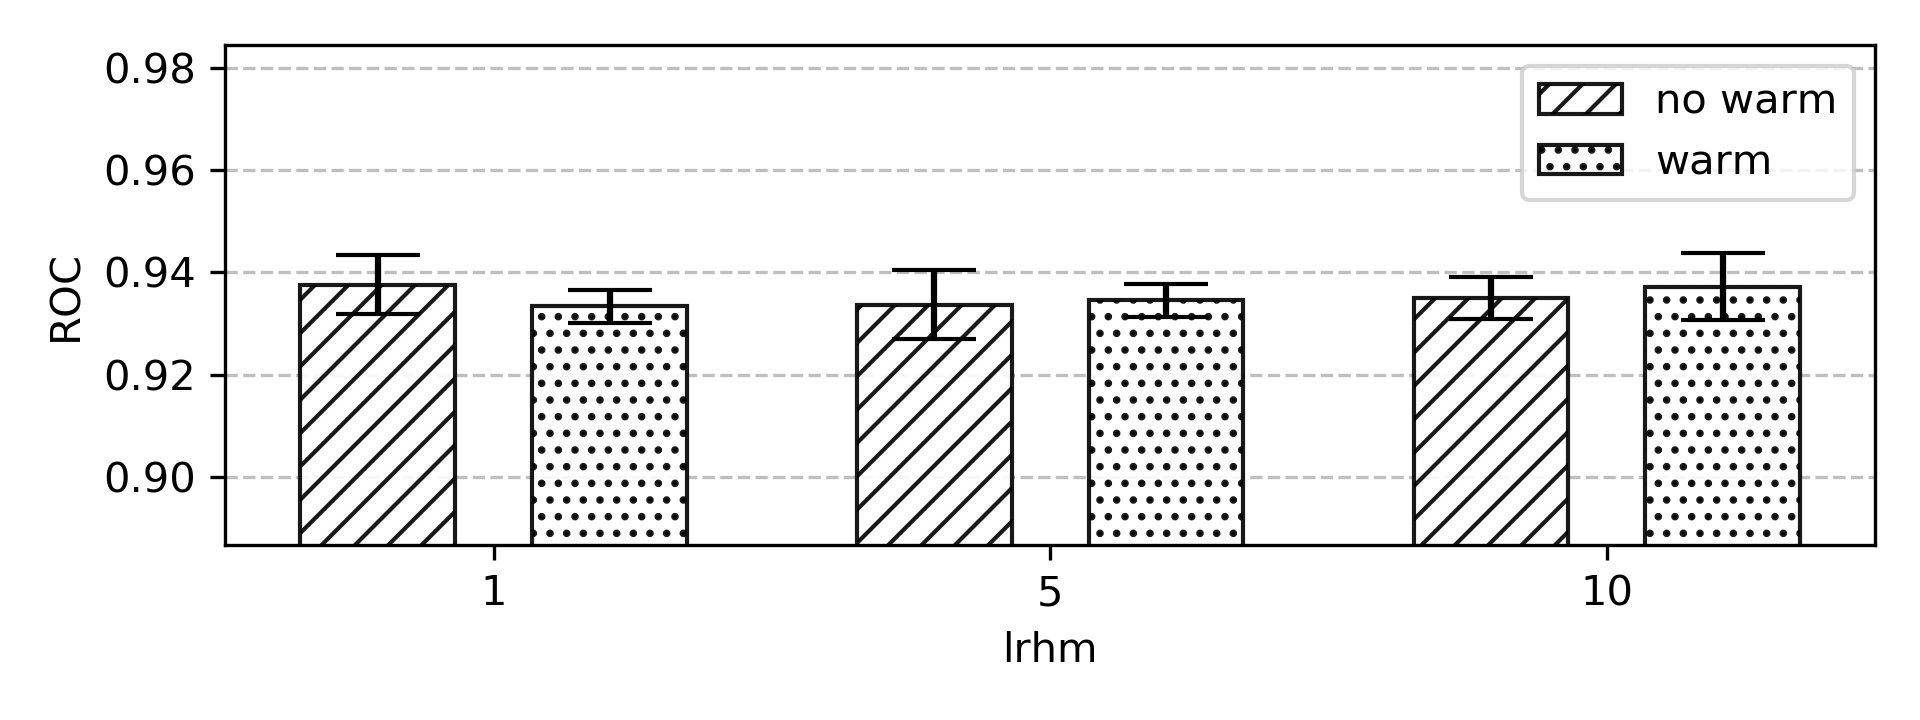
\includegraphics[width=\textwidth]{mtask/supp/bar_lrhm_1e-4_densenet121_ulg_breast2.png}
    \caption{Breast2}
  \end{subfigure}
  \begin{subfigure}{0.48\textwidth}
    \centering
    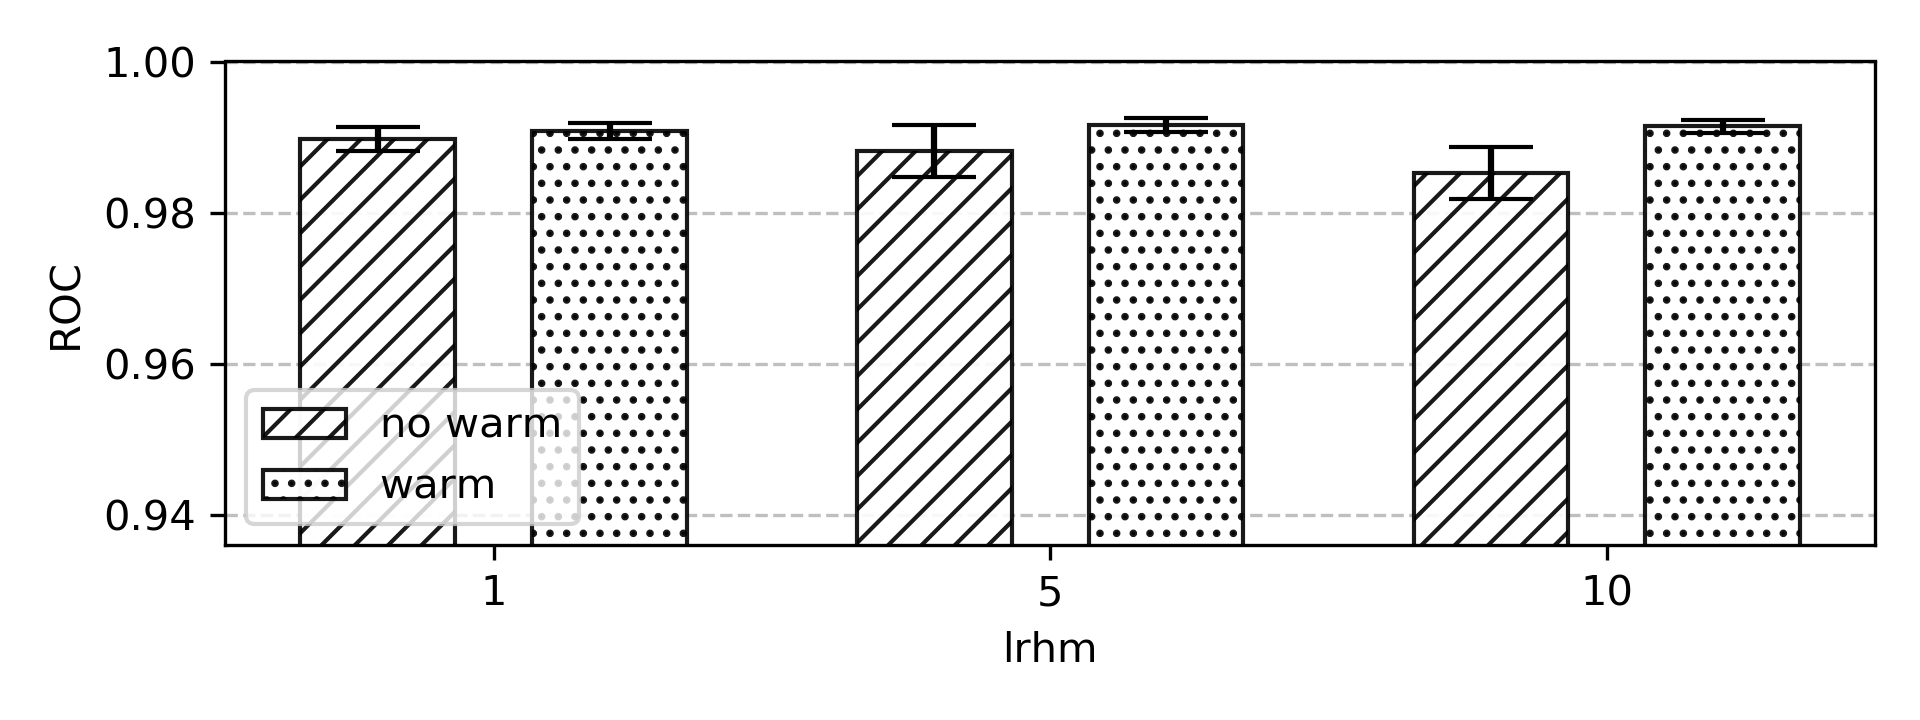
\includegraphics[width=\textwidth]{mtask/supp/bar_lrhm_1e-4_densenet121_ulg_lbtd2_chimio_necrose.png}\\
    \caption{Necrose}
  \end{subfigure}
  \begin{subfigure}{0.48\textwidth}
    \centering
    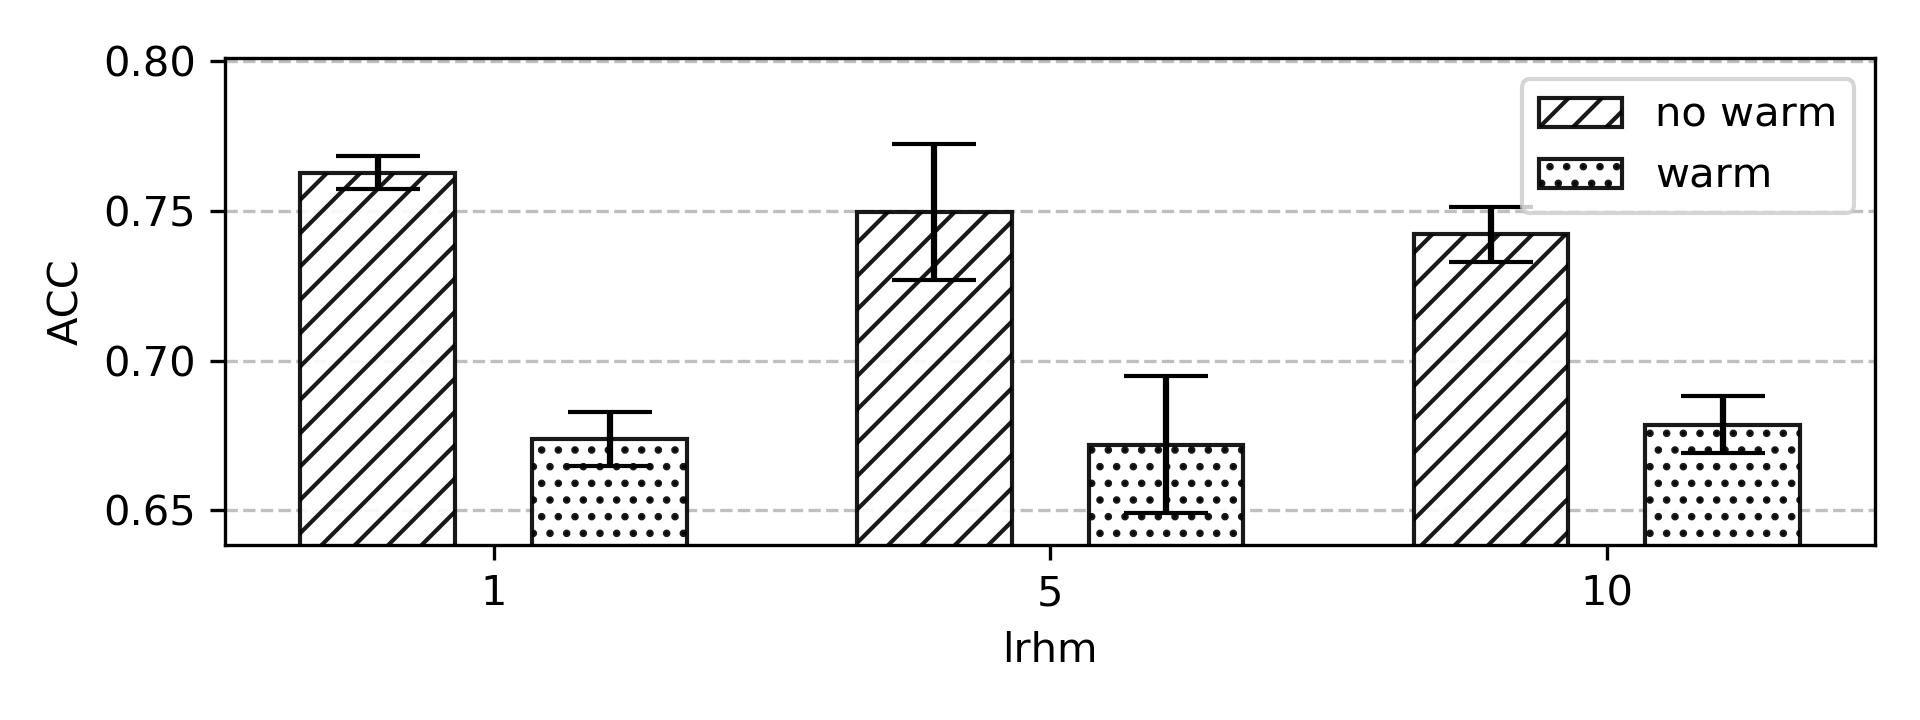
\includegraphics[width=\textwidth]{mtask/supp/bar_lrhm_1e-4_densenet121_ulg_lbtd_lba.png}
    \caption{MouseLba}
  \end{subfigure}
  \begin{subfigure}{0.48\textwidth}
    \centering
    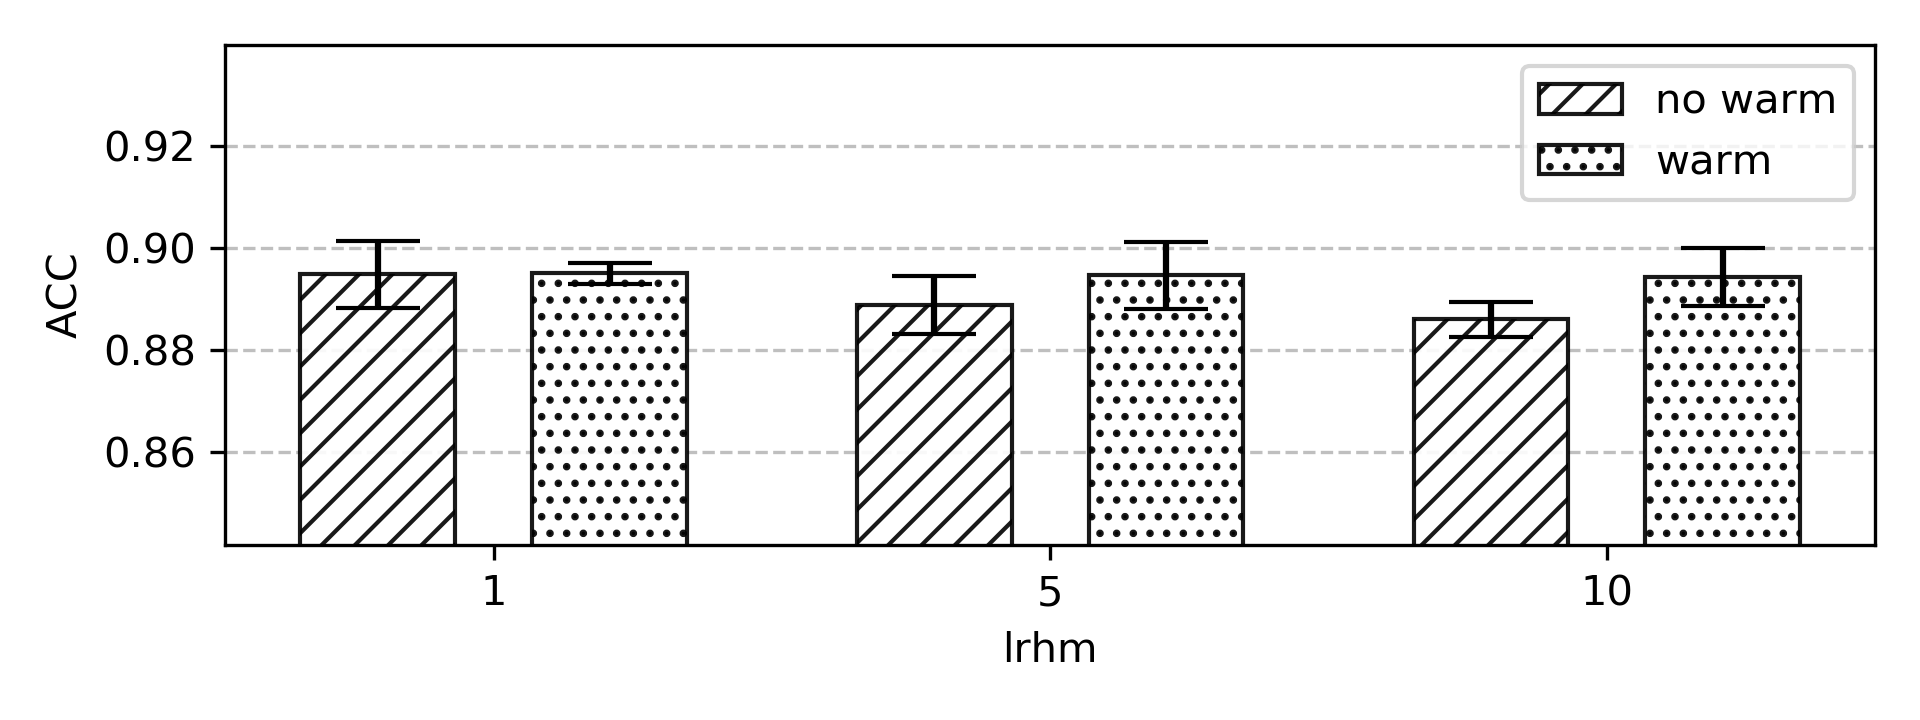
\includegraphics[width=\textwidth]{mtask/supp/bar_lrhm_1e-4_densenet121_ulg_lbtd_tissus.png}
    \caption{Lung}
  \end{subfigure}
  \caption{Transfer performance for combinations of the hyperparameters $\gamma_\tau$ (learning rate heads multiplier) and $w$ (warm up) with learning rate $\gamma = 10^{-4}$ on DenseNet121.}
  \label{app:mtask:fig:bar_lrhm_densenet}
\end{figure*}

\begin{figure*}[h]
  \centering
  \begin{subfigure}{0.48\textwidth}
    \centering
    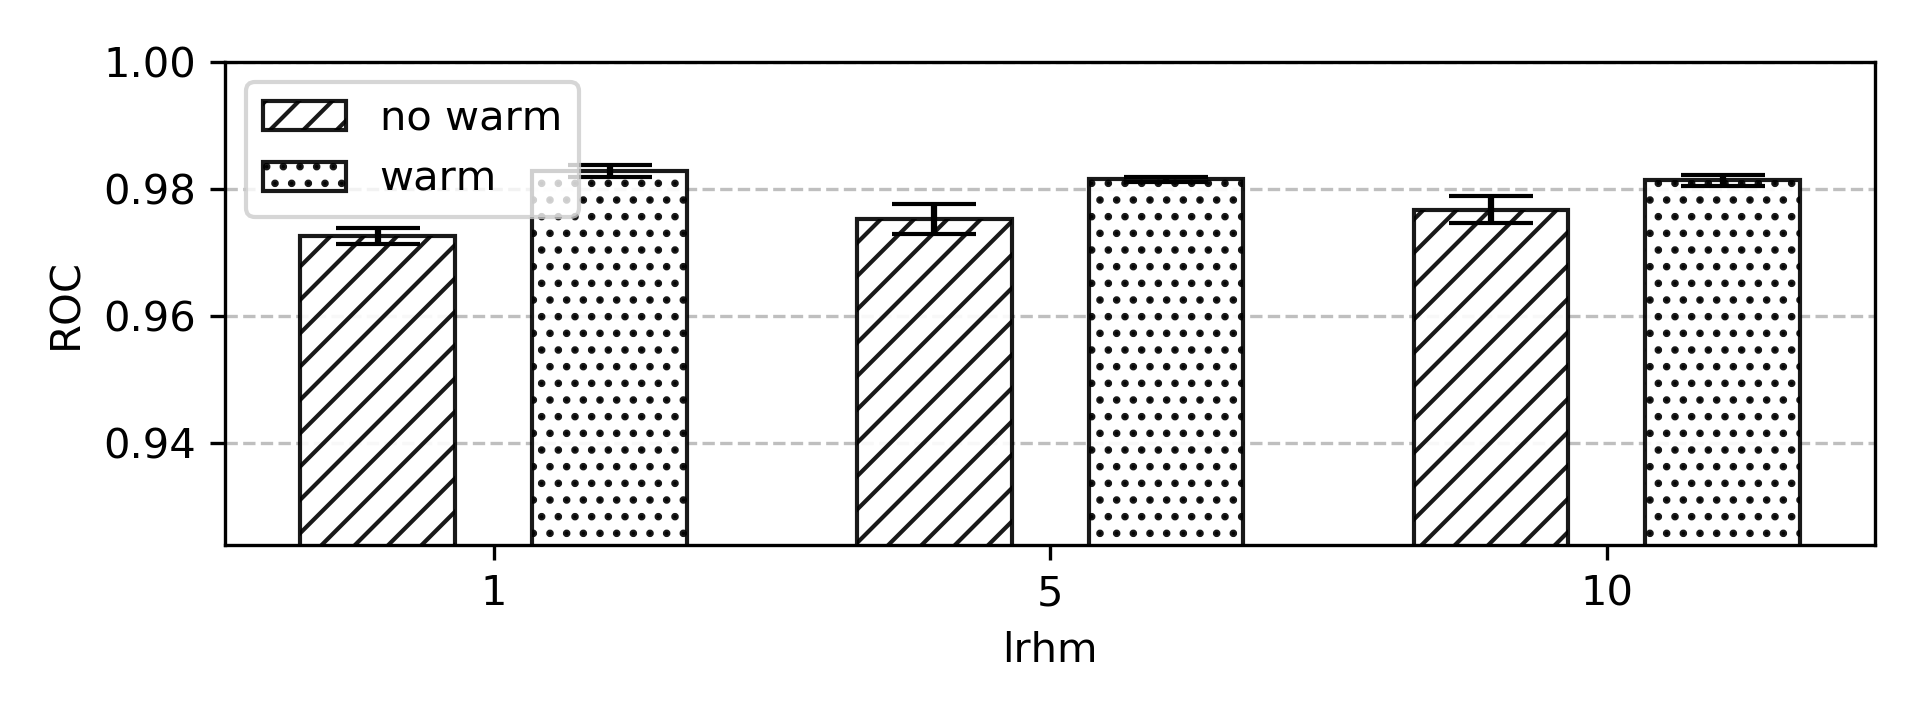
\includegraphics[width=\textwidth]{mtask/supp/bar_lrhm_1e-4_resnet50_cells_no_aug.png}
    \caption{CellInclusion}
  \end{subfigure}
  \begin{subfigure}{0.48\textwidth}
    \centering
    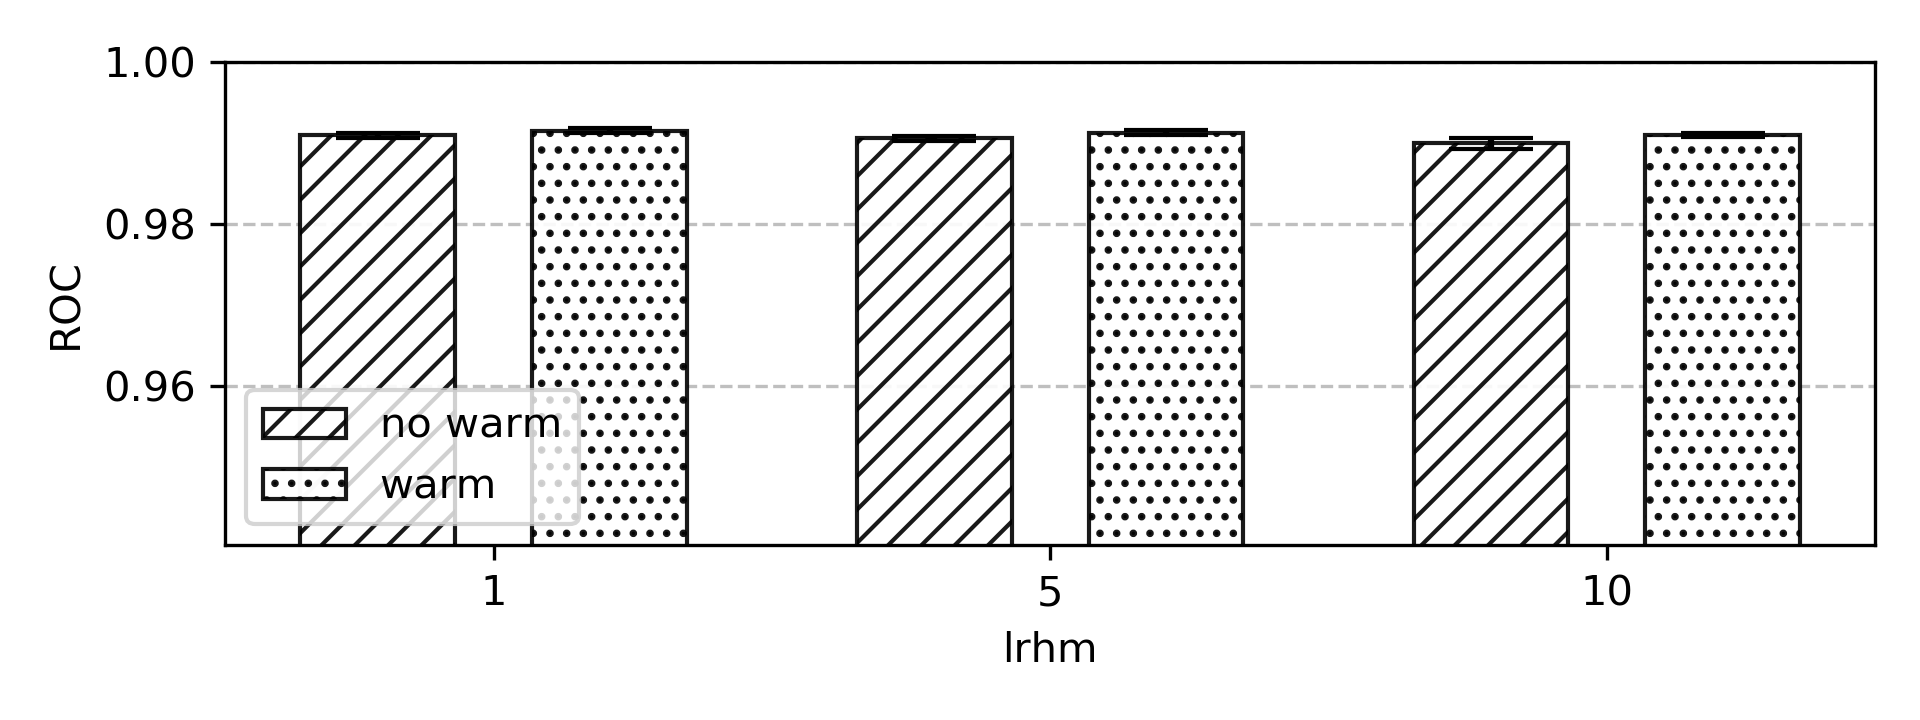
\includegraphics[width=\textwidth]{mtask/supp/bar_lrhm_1e-4_resnet50_glomeruli_no_aug.png}\\
    \caption{Glomeruli}
  \end{subfigure}
  \begin{subfigure}{0.48\textwidth}
    \centering
    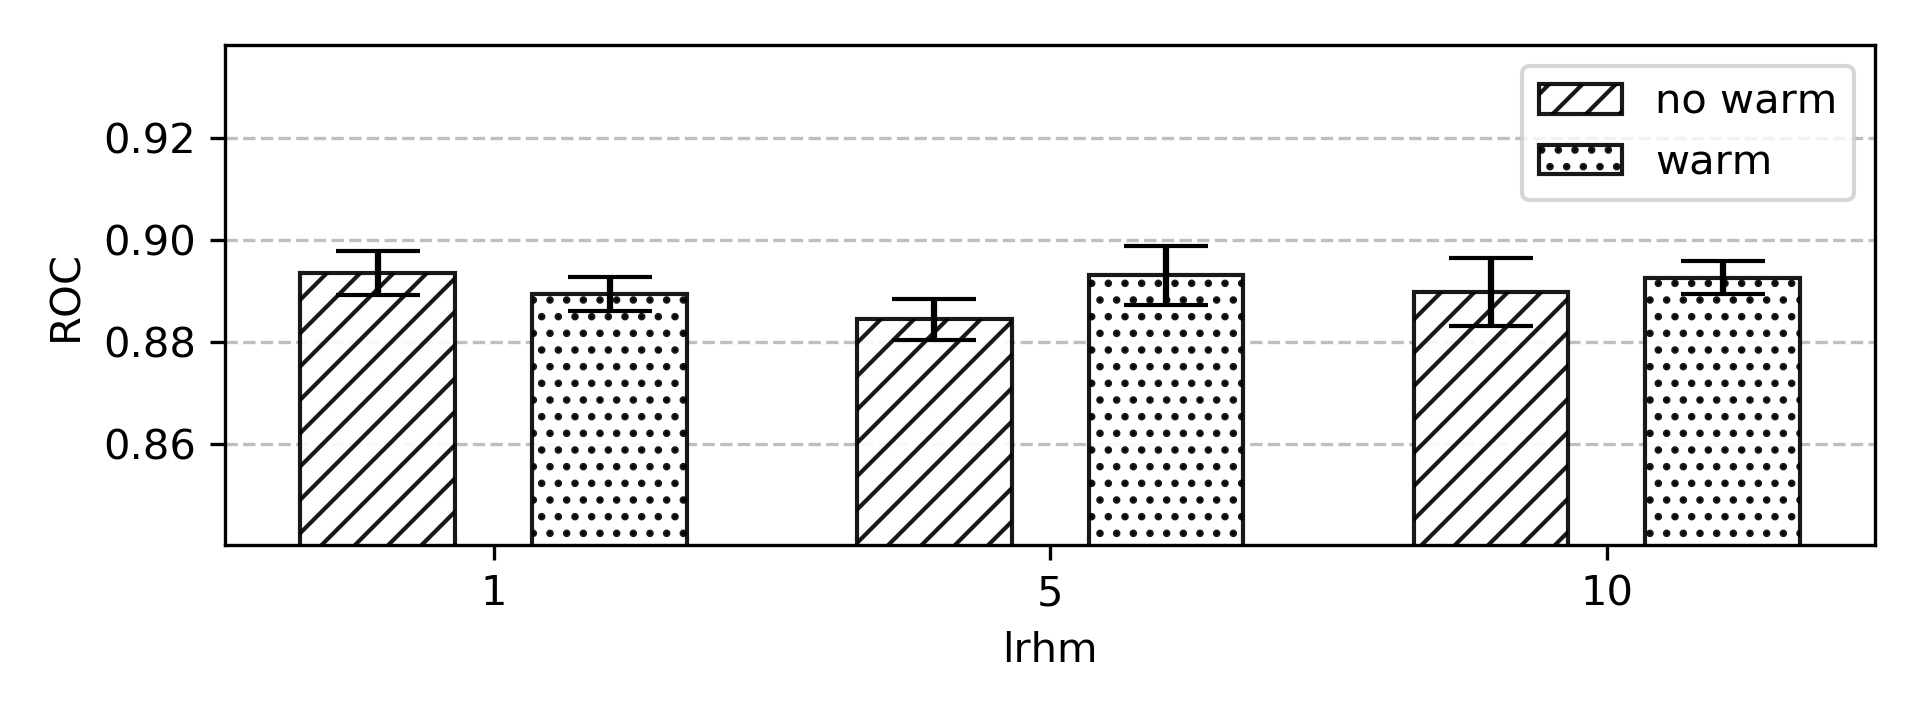
\includegraphics[width=\textwidth]{mtask/supp/bar_lrhm_1e-4_resnet50_patterns_no_aug.png}
    \caption{ProliferativePattern}
  \end{subfigure}
  \begin{subfigure}{0.48\textwidth}
    \centering
    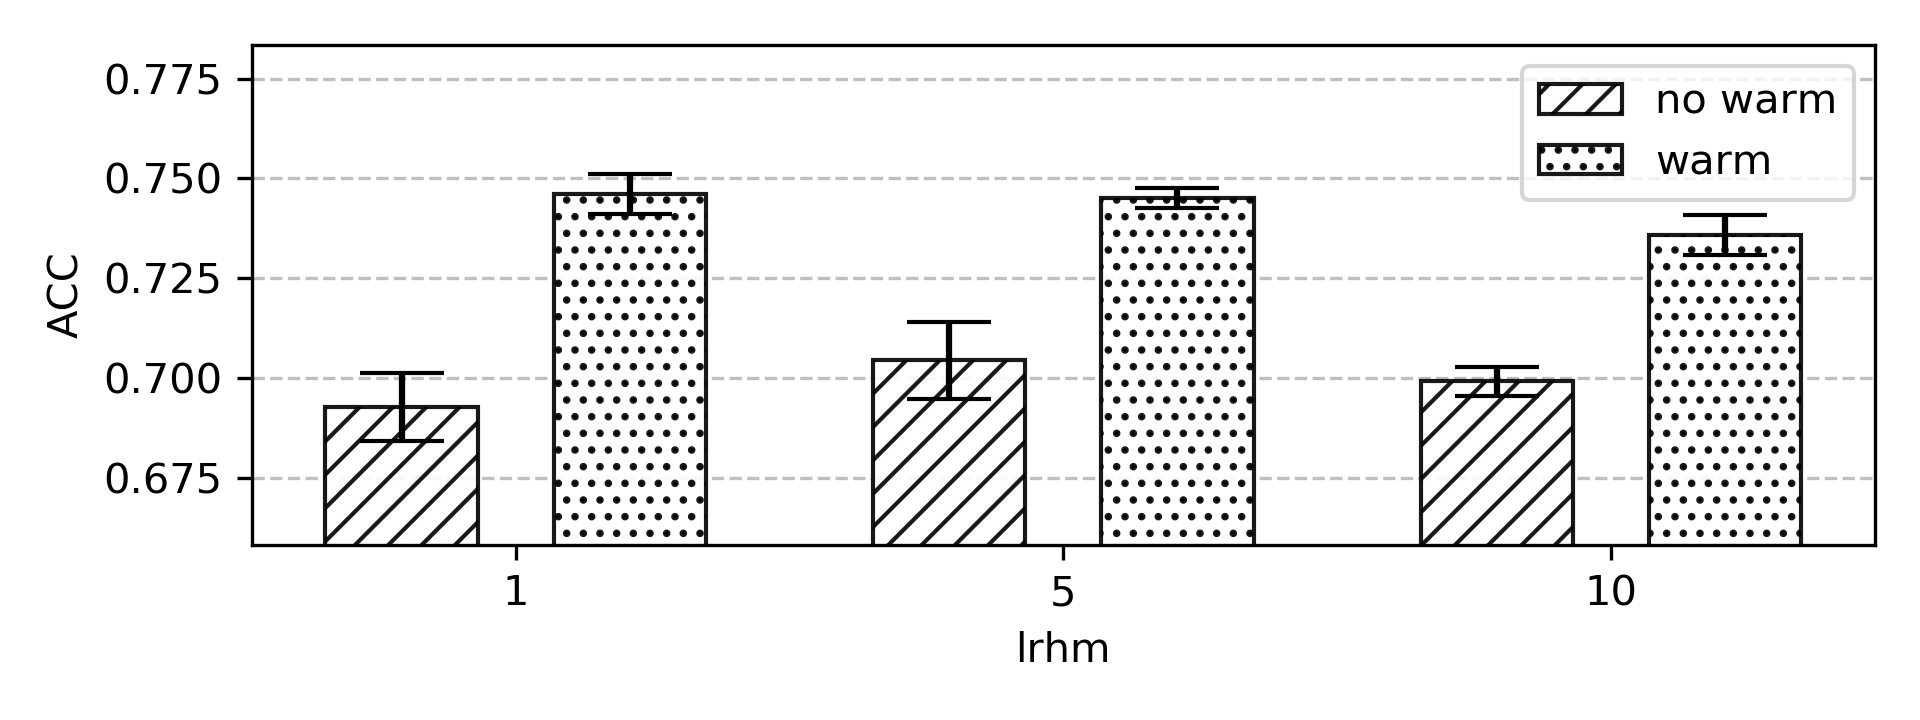
\includegraphics[width=\textwidth]{mtask/supp/bar_lrhm_1e-4_resnet50_ulb_anapath_lba.png}\\
    \caption{HumanLba}
  \end{subfigure}
  \begin{subfigure}{0.48\textwidth}
    \centering
    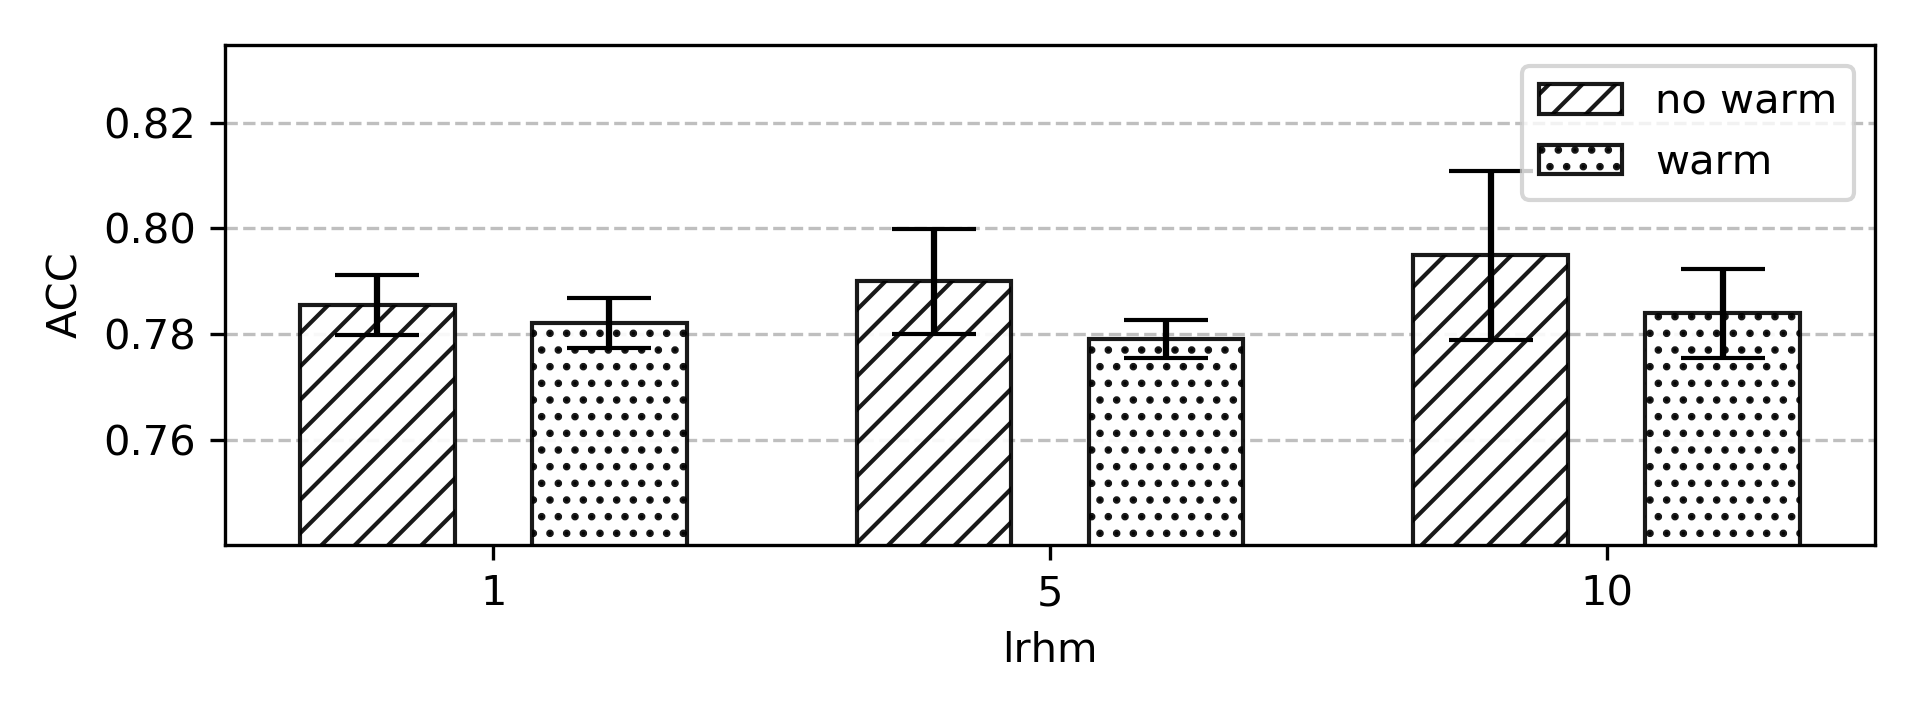
\includegraphics[width=\textwidth]{mtask/supp/bar_lrhm_1e-4_resnet50_ulg_bonemarrow.png}
    \caption{BoneMarrow}
  \end{subfigure}
  \begin{subfigure}{0.48\textwidth}
    \centering
    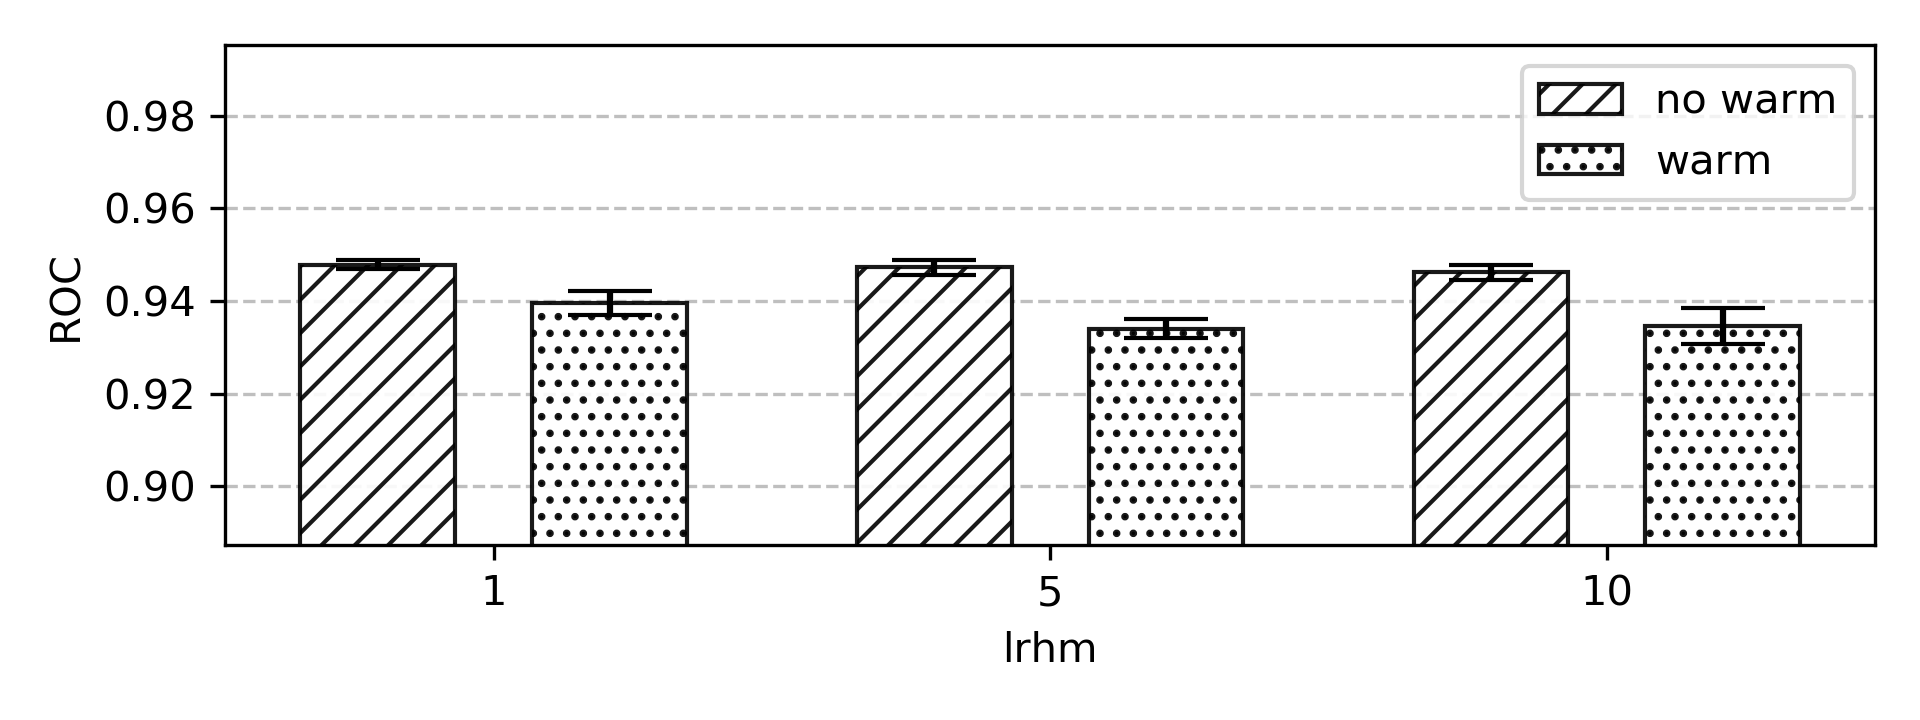
\includegraphics[width=\textwidth]{mtask/supp/bar_lrhm_1e-4_resnet50_ulg_breast.png}\\
    \caption{Breast1}
  \end{subfigure}
  \begin{subfigure}{0.48\textwidth}
    \centering
    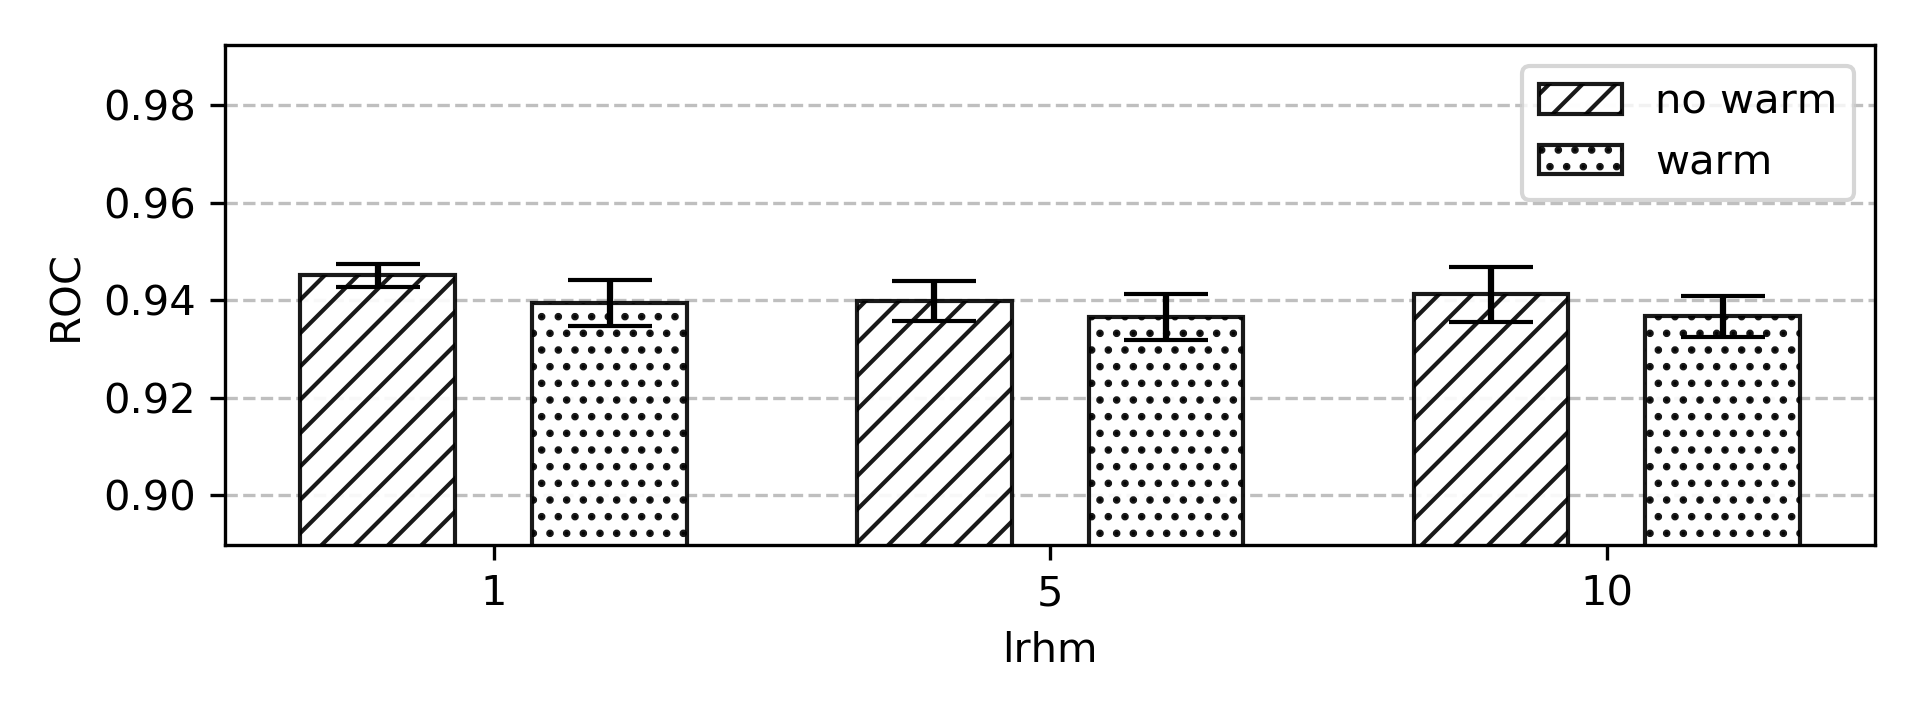
\includegraphics[width=\textwidth]{mtask/supp/bar_lrhm_1e-4_resnet50_ulg_breast2.png}
    \caption{Breast2}
  \end{subfigure}
  \begin{subfigure}{0.48\textwidth}
    \centering
    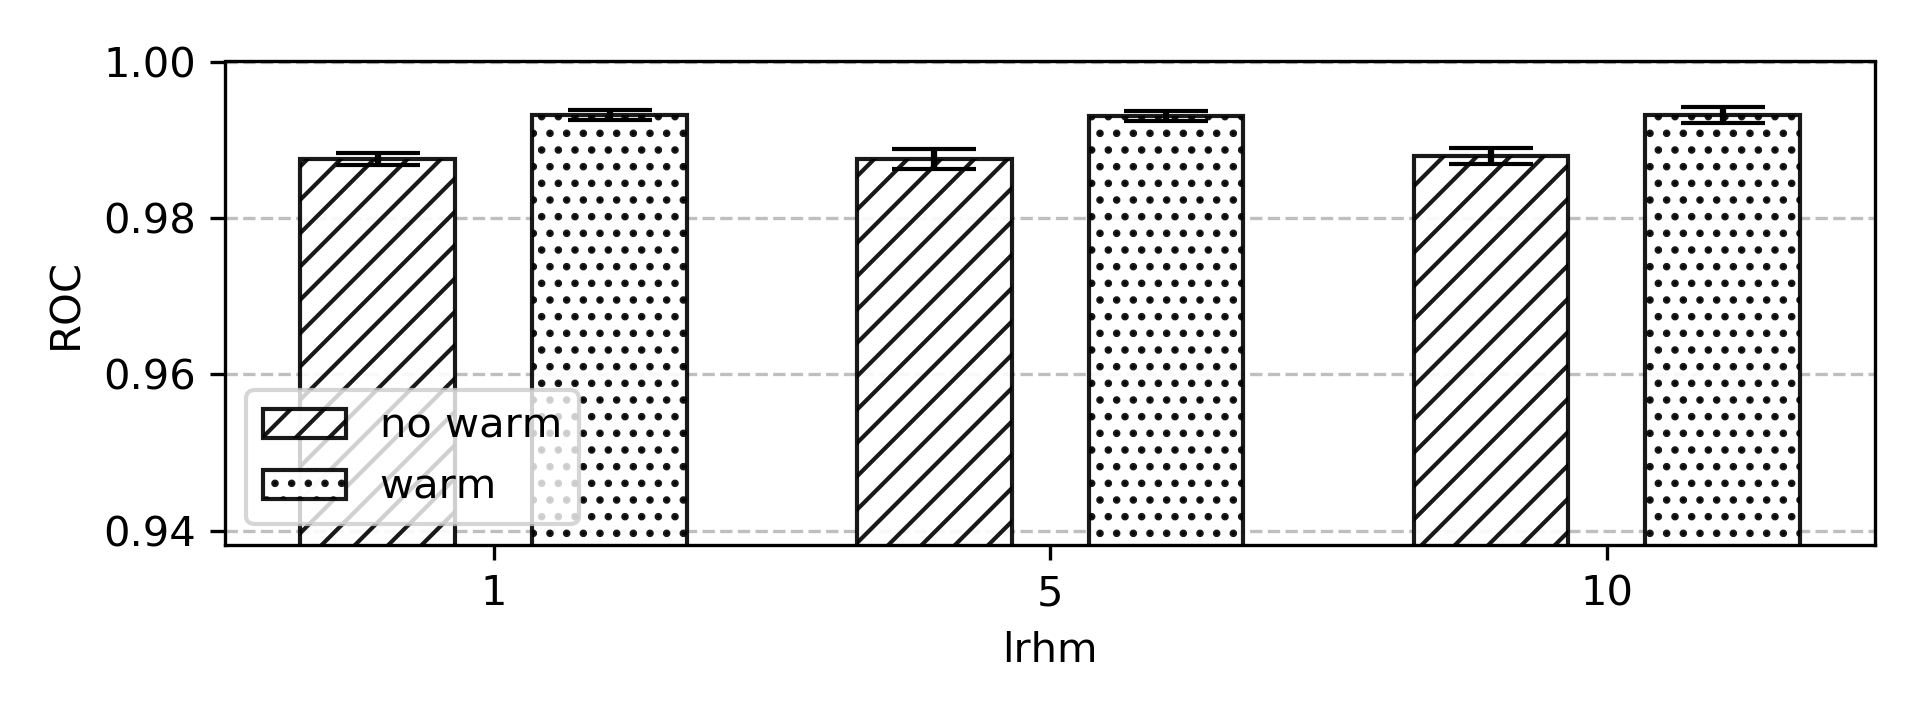
\includegraphics[width=\textwidth]{mtask/supp/bar_lrhm_1e-4_resnet50_ulg_lbtd2_chimio_necrose.png}\\
    \caption{Necrose}
  \end{subfigure}
  \begin{subfigure}{0.48\textwidth}
    \centering
    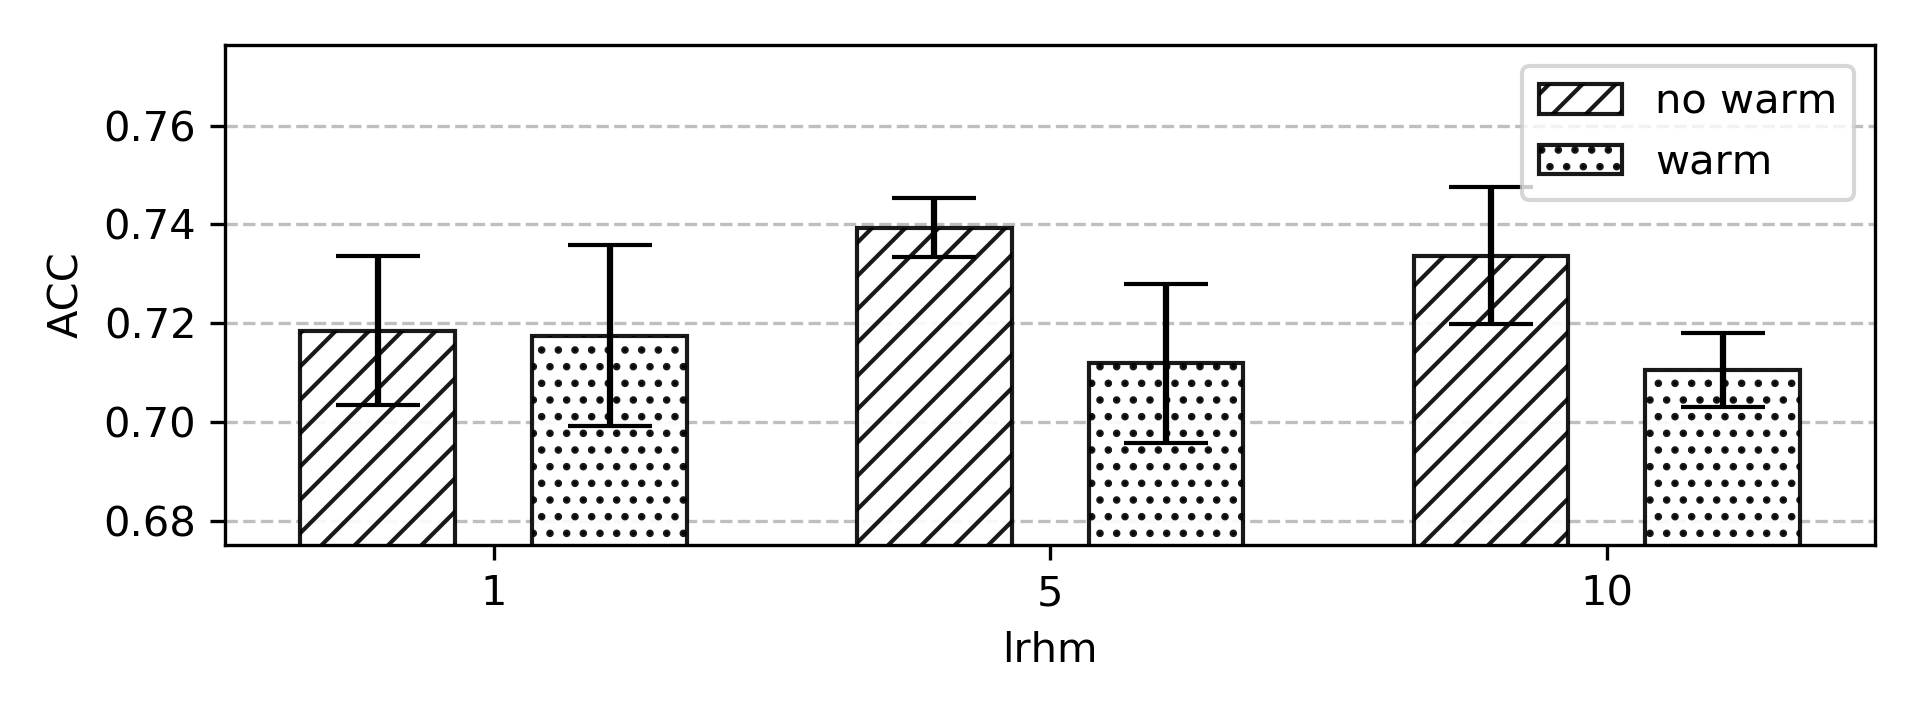
\includegraphics[width=\textwidth]{mtask/supp/bar_lrhm_1e-4_resnet50_ulg_lbtd_lba.png}
    \caption{MouseLba}
  \end{subfigure}
  \begin{subfigure}{0.48\textwidth}
    \centering
    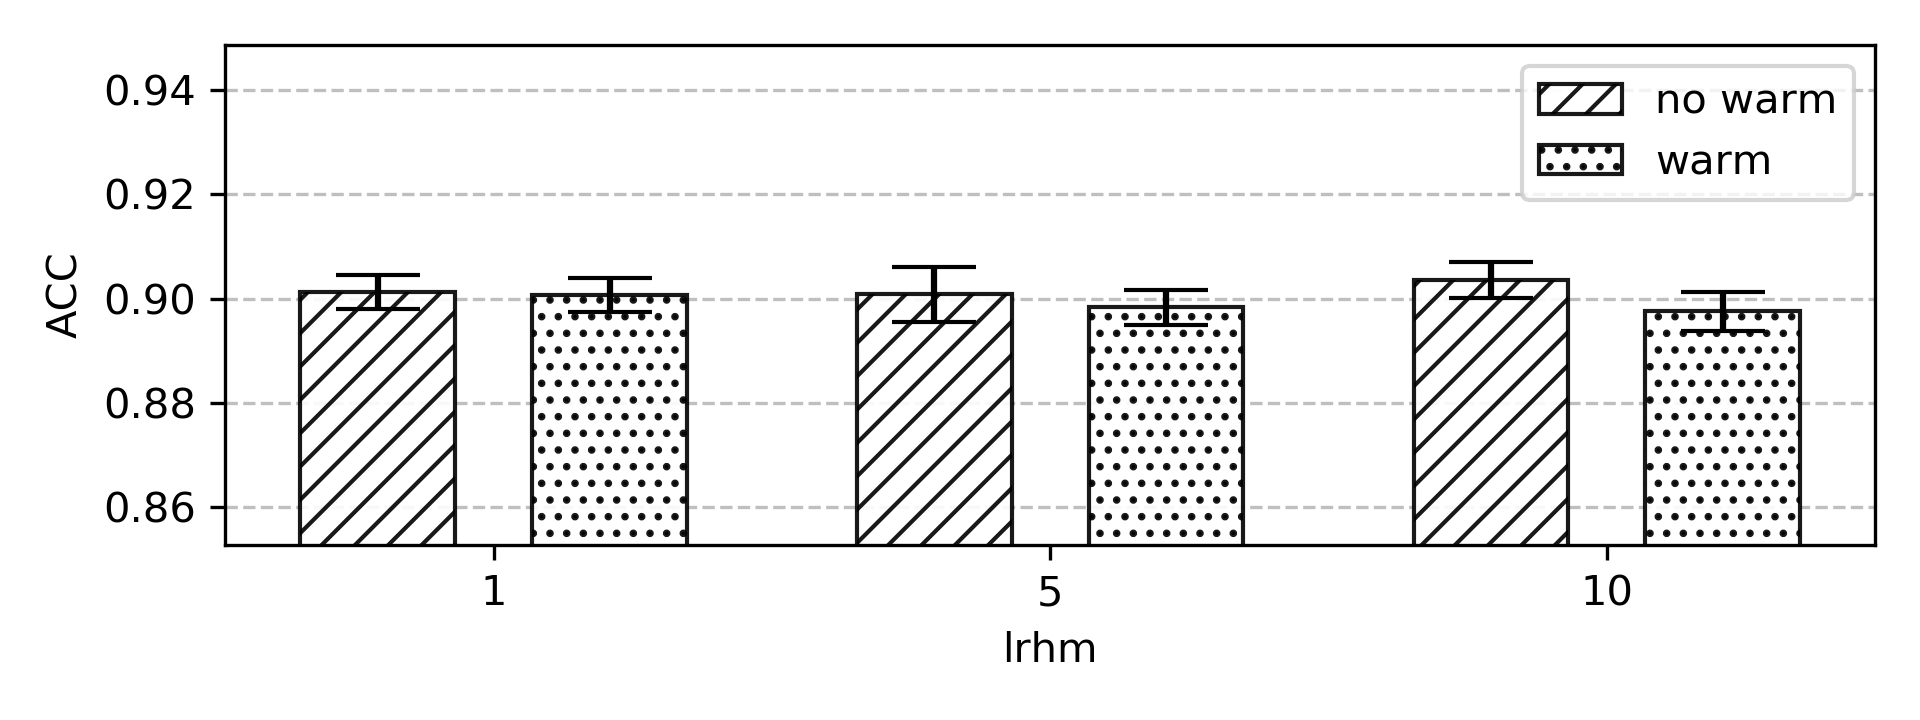
\includegraphics[width=\textwidth]{mtask/supp/bar_lrhm_1e-4_resnet50_ulg_lbtd_tissus.png}
    \caption{Lung}
  \end{subfigure}
  \caption{Transfer performance for combinations of the hyperparameters $\gamma_\tau$ (learning rate heads multiplier) and $w$ (warm up) with learning rate $\gamma = 10^{-4}$ on ResNet50.}
  \label{app:mtask:fig:bar_lrhm_resnet}
\end{figure*}

\begin{figure*}[h]
  \centering
  \begin{subfigure}{0.48\textwidth}
    \centering
    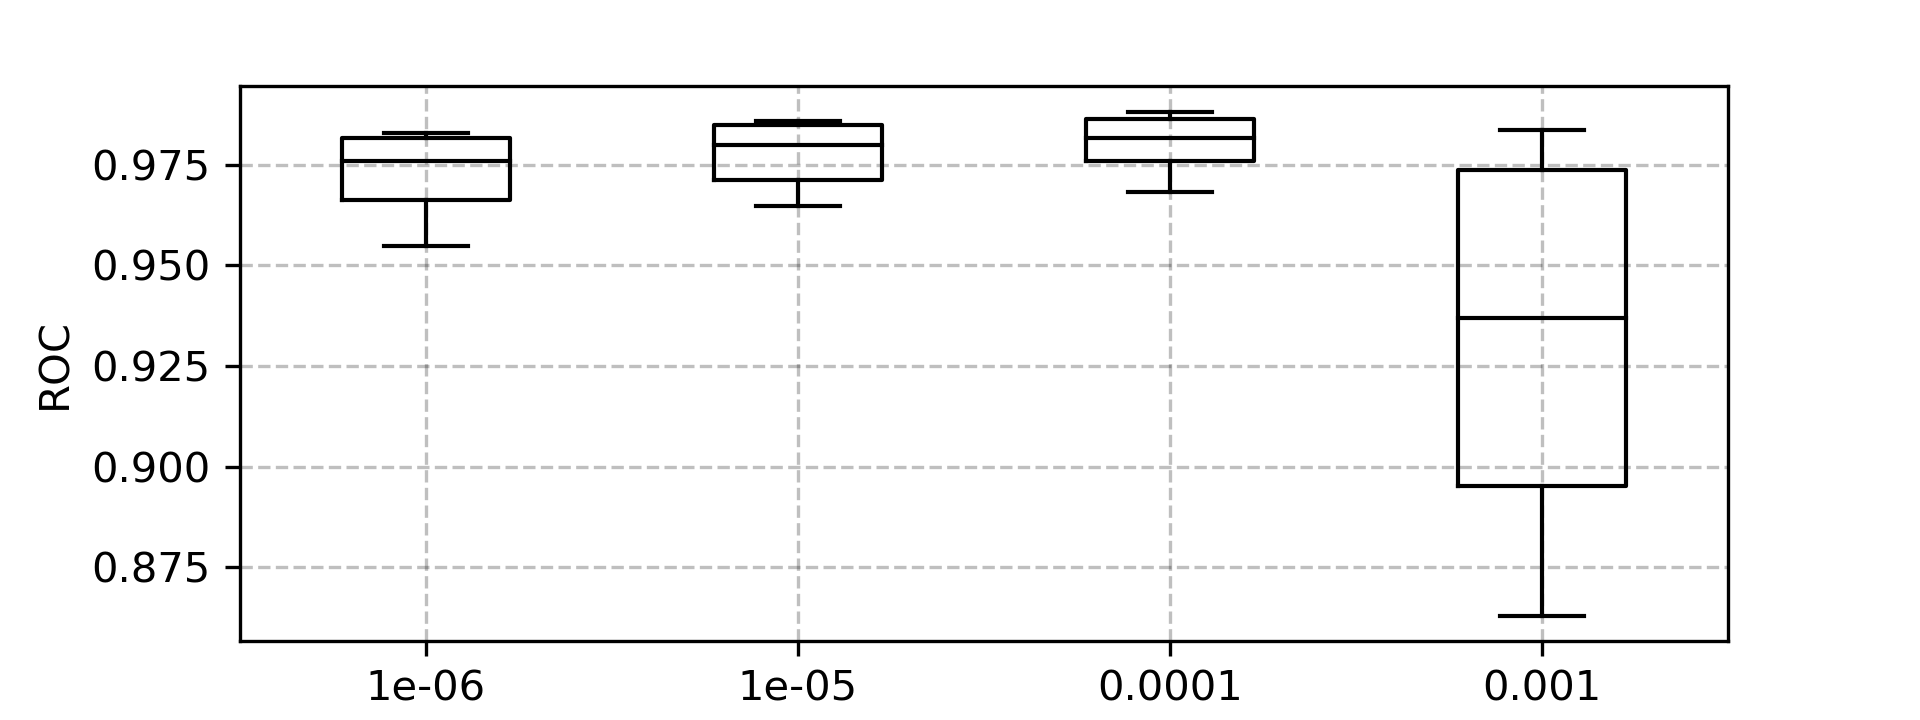
\includegraphics[width=\textwidth]{mtask/supp/densenet121_cells_no_aug_learning_rate.png}
    \caption{CellInclusion}
    \end{subfigure}
  \begin{subfigure}{0.48\textwidth}
    \centering
    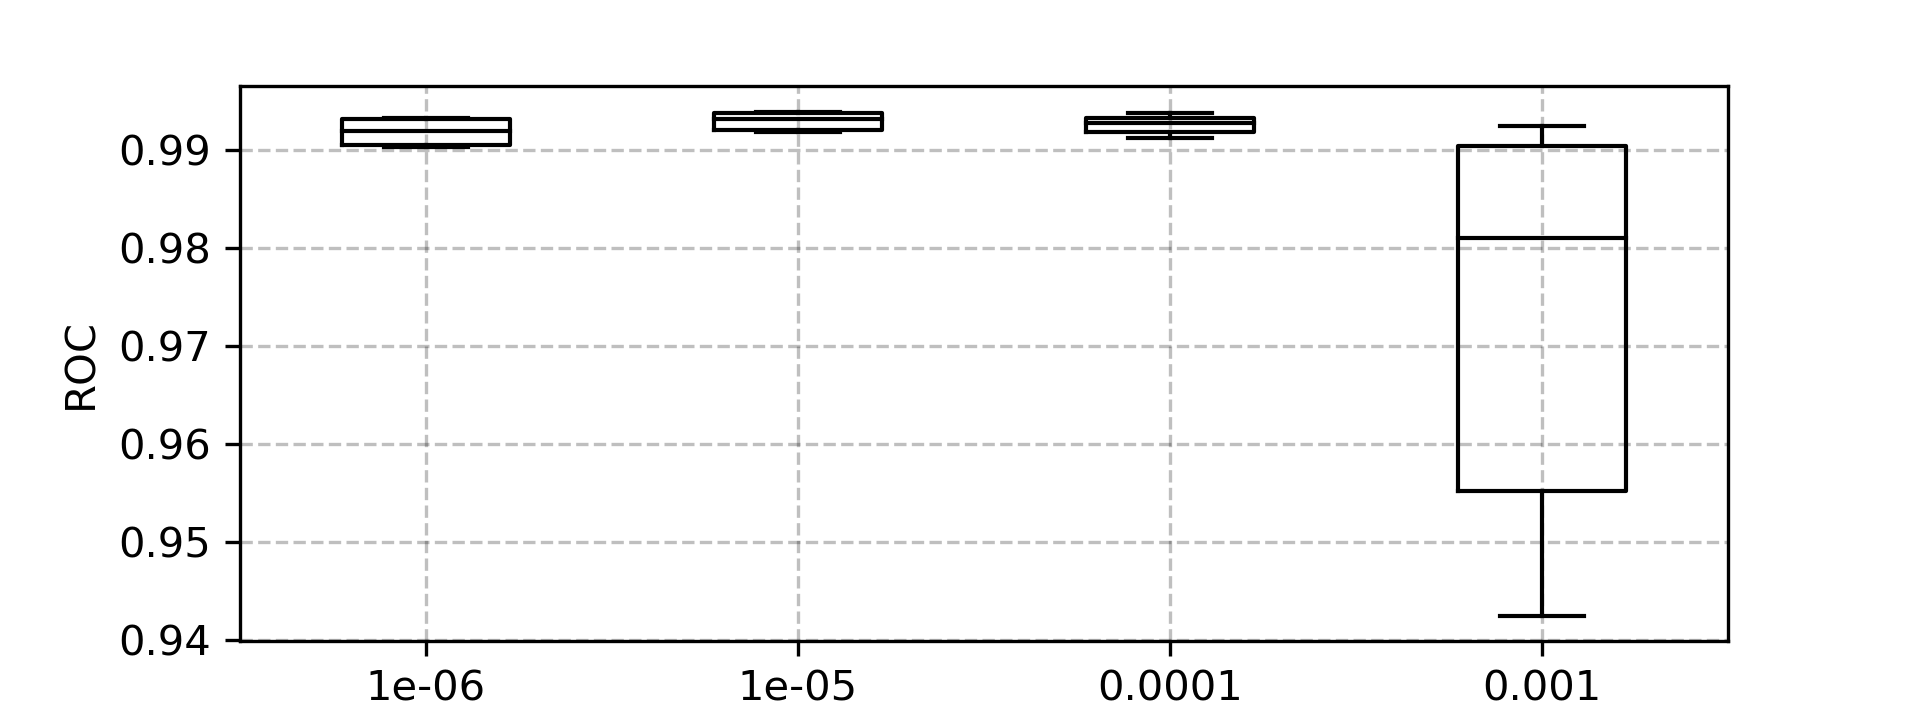
\includegraphics[width=\textwidth]{mtask/supp/densenet121_glomeruli_no_aug_learning_rate.png}\\
    \caption{Glomeruli}
  \end{subfigure}
  \begin{subfigure}{0.48\textwidth}
    \centering
    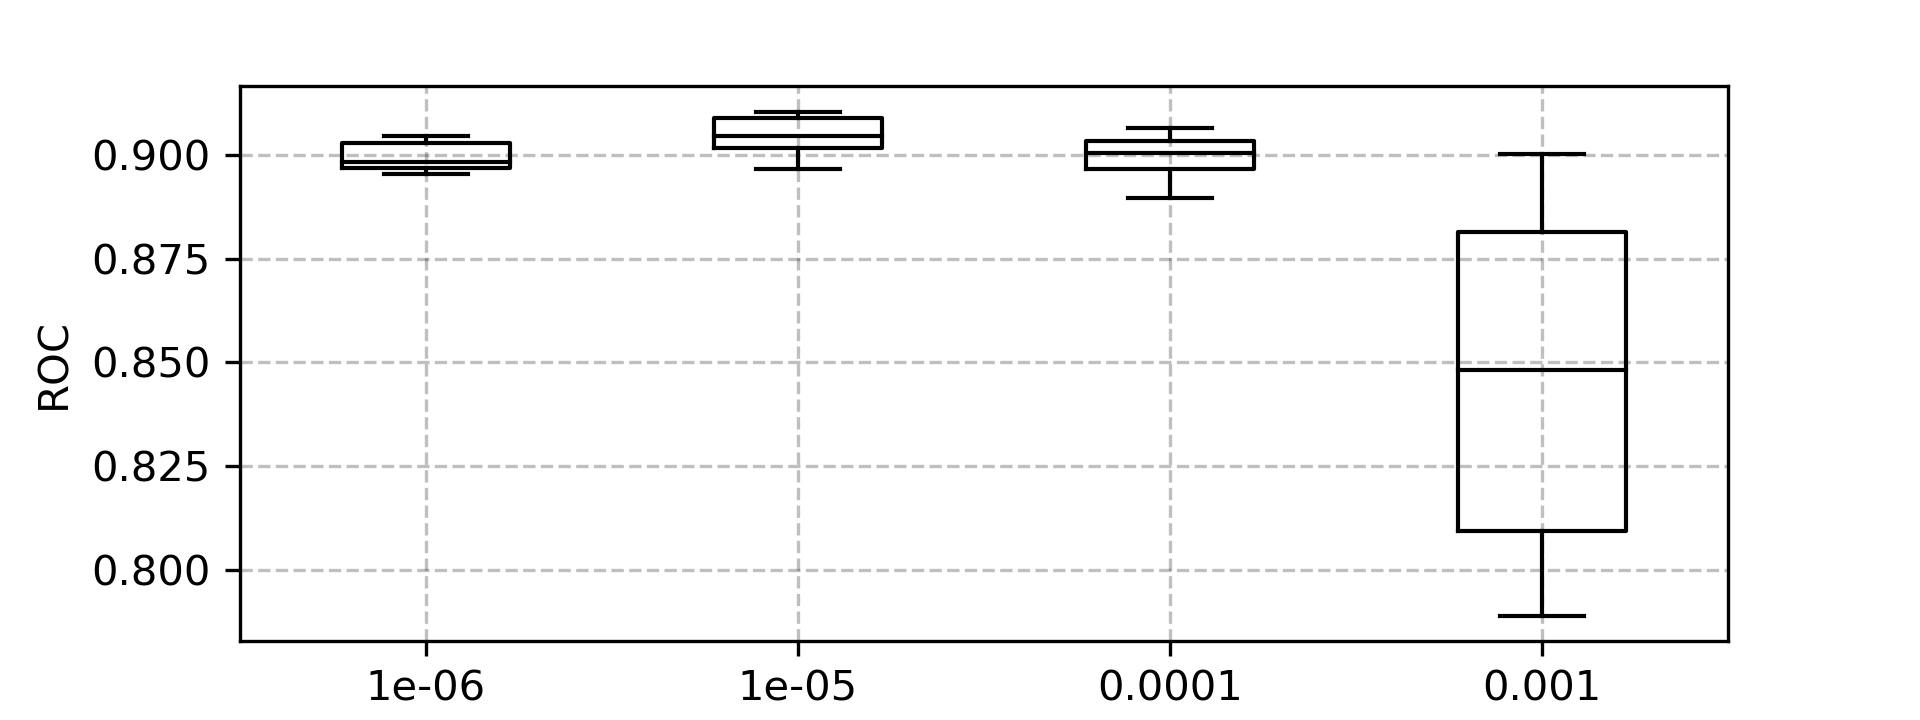
\includegraphics[width=\textwidth]{mtask/supp/densenet121_patterns_no_aug_learning_rate.png}
    \caption{ProliferativePattern}
  \end{subfigure}
  \begin{subfigure}{0.48\textwidth}
    \centering
    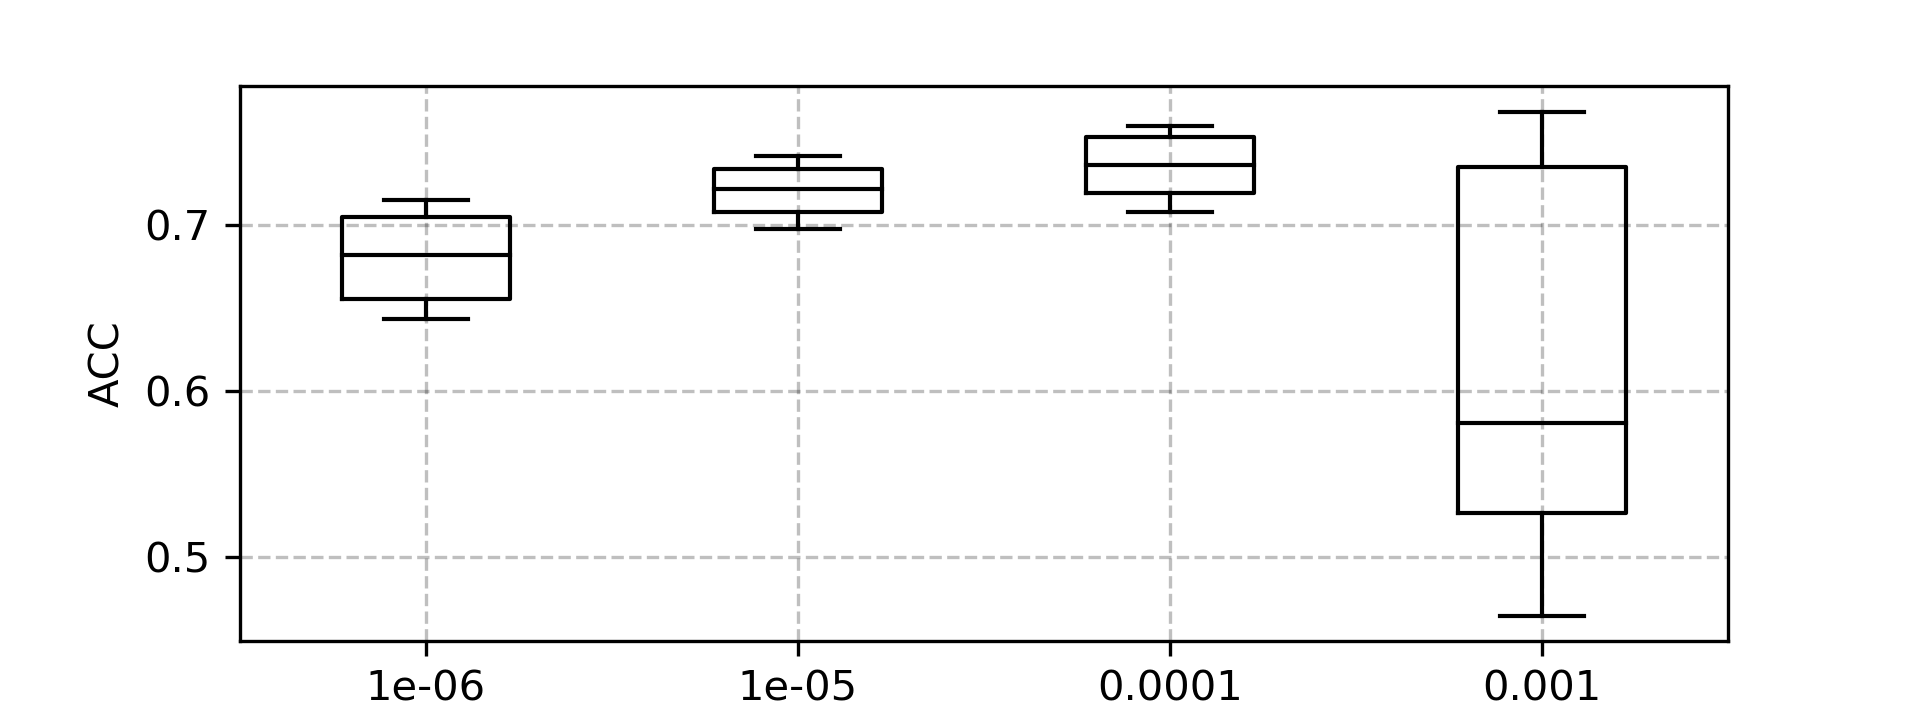
\includegraphics[width=\textwidth]{mtask/supp/densenet121_ulb_anapath_lba_learning_rate.png}\\
    \caption{HumanLba}
  \end{subfigure}
  \begin{subfigure}{0.48\textwidth}
    \centering
    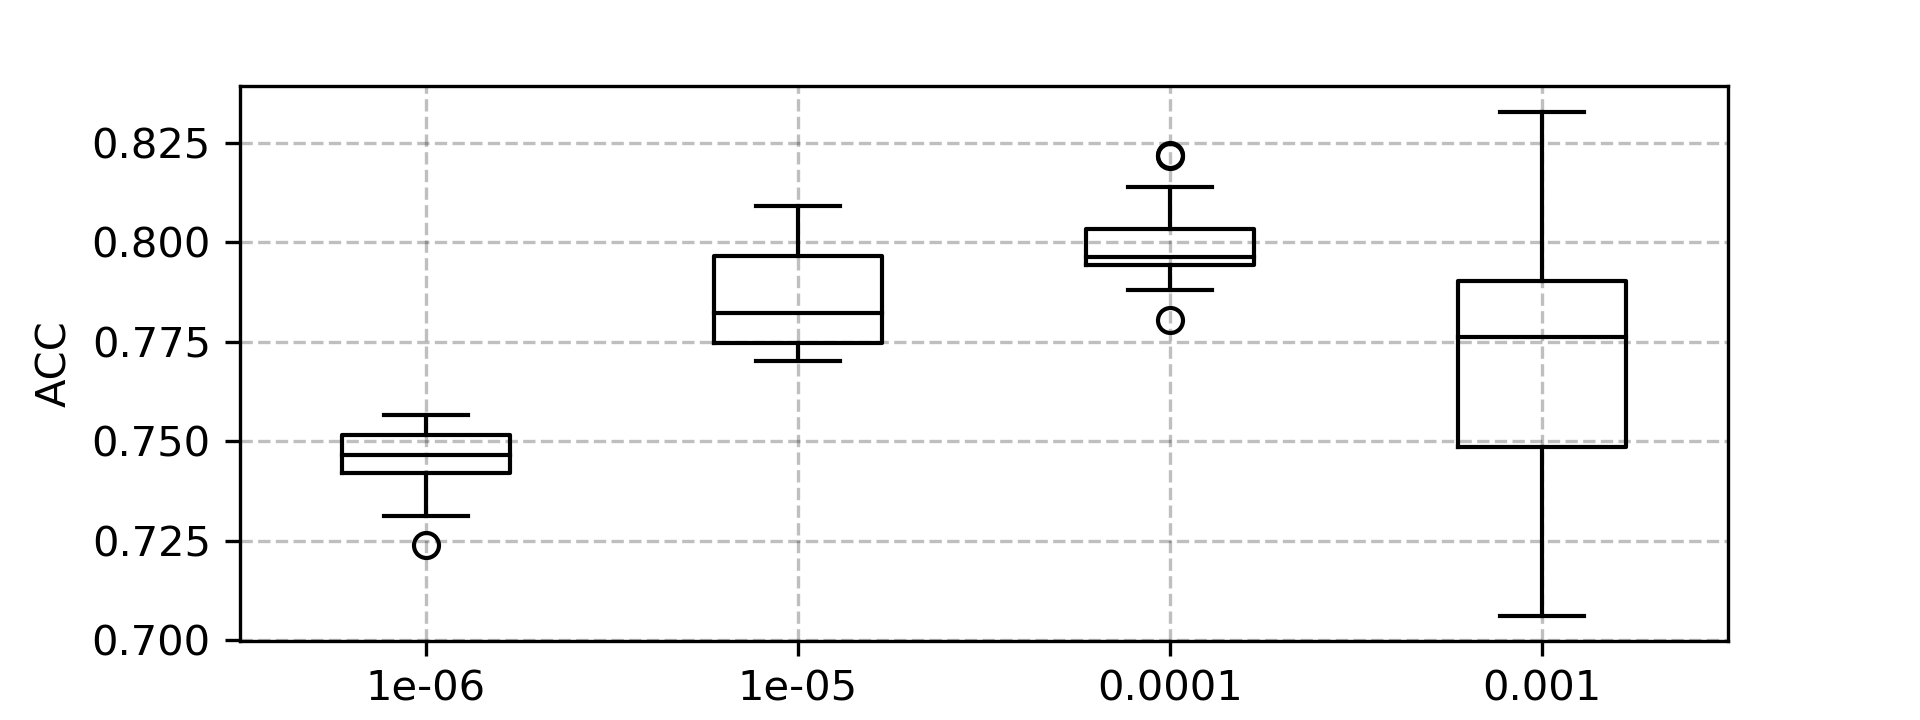
\includegraphics[width=\textwidth]{mtask/supp/densenet121_ulg_bonemarrow_learning_rate.png}
    \caption{BoneMarrow}
  \end{subfigure}
  \begin{subfigure}{0.48\textwidth}
    \centering
    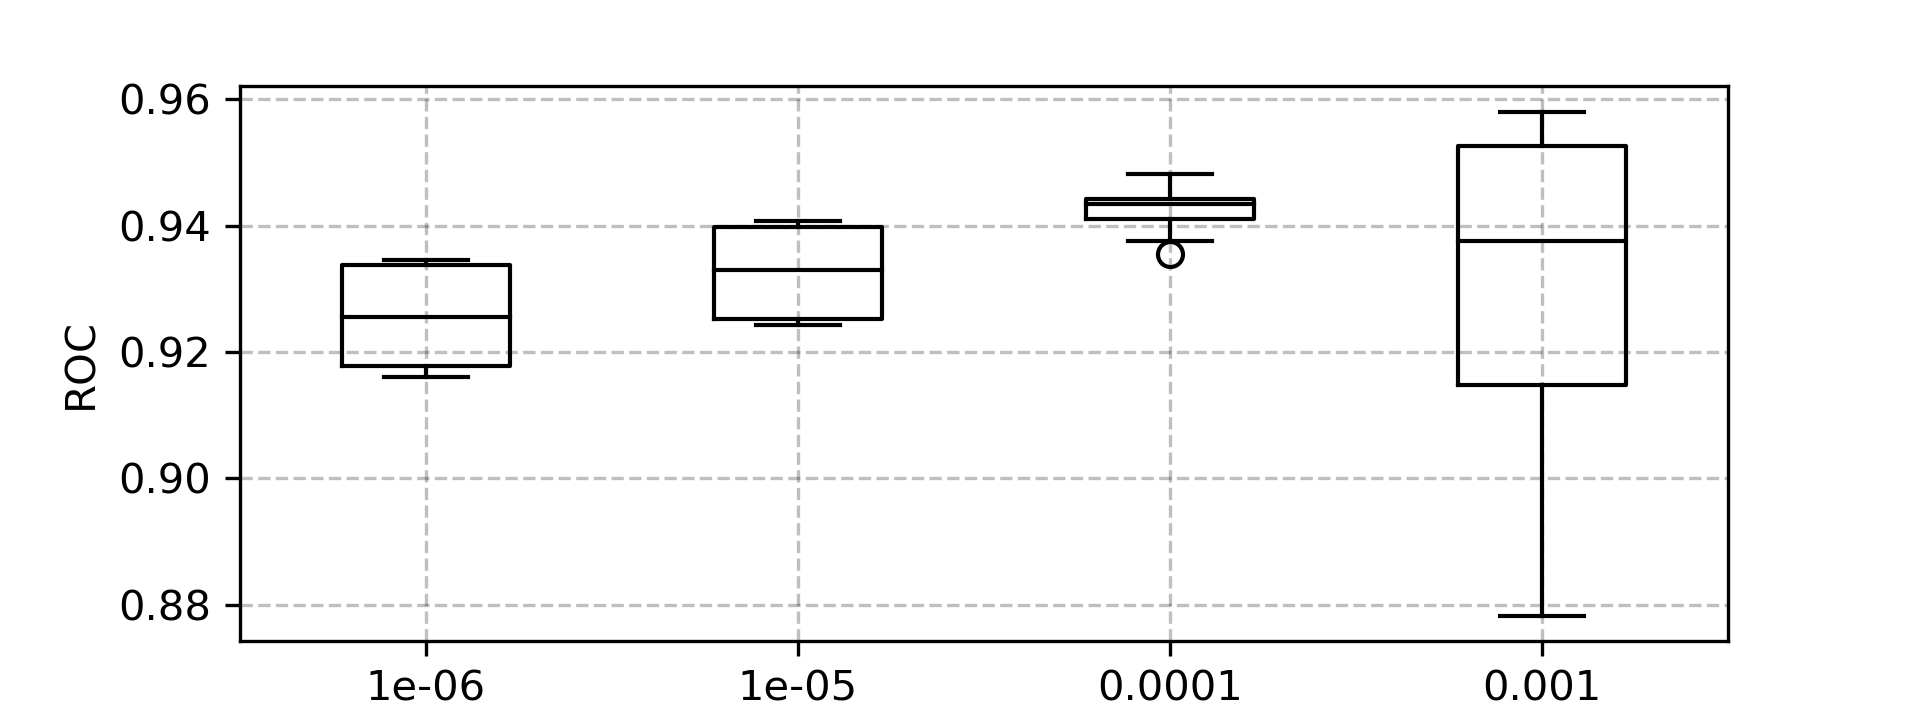
\includegraphics[width=\textwidth]{mtask/supp/densenet121_ulg_breast_learning_rate.png}\\
    \caption{Breast1}
  \end{subfigure}
  \begin{subfigure}{0.48\textwidth}
    \centering
    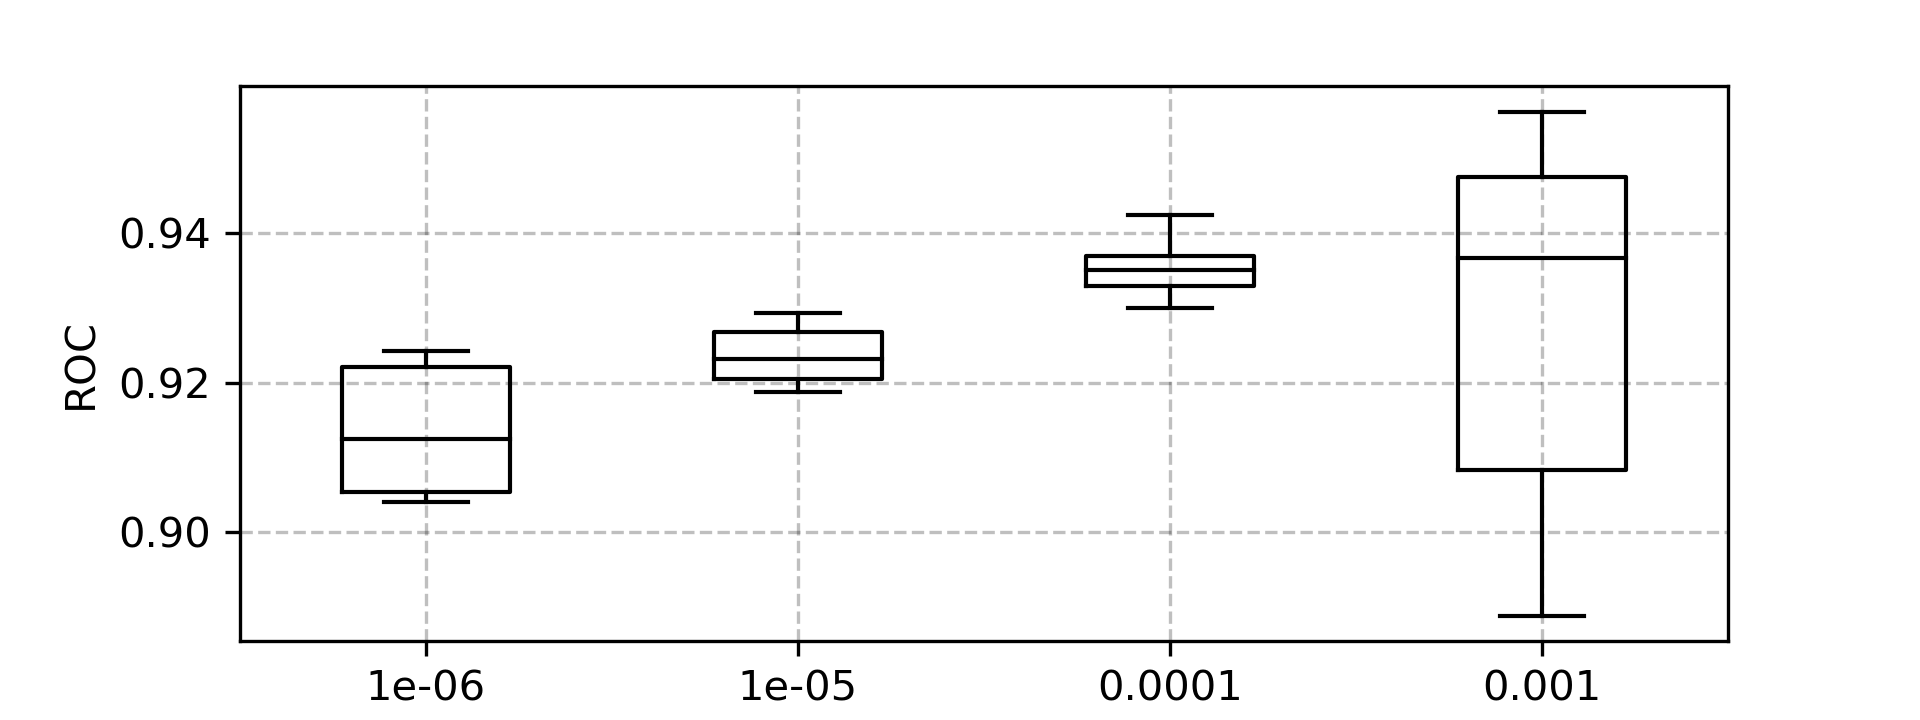
\includegraphics[width=\textwidth]{mtask/supp/densenet121_ulg_breast2_learning_rate.png}
    \caption{Breast2}
  \end{subfigure}
  \begin{subfigure}{0.48\textwidth}
    \centering
    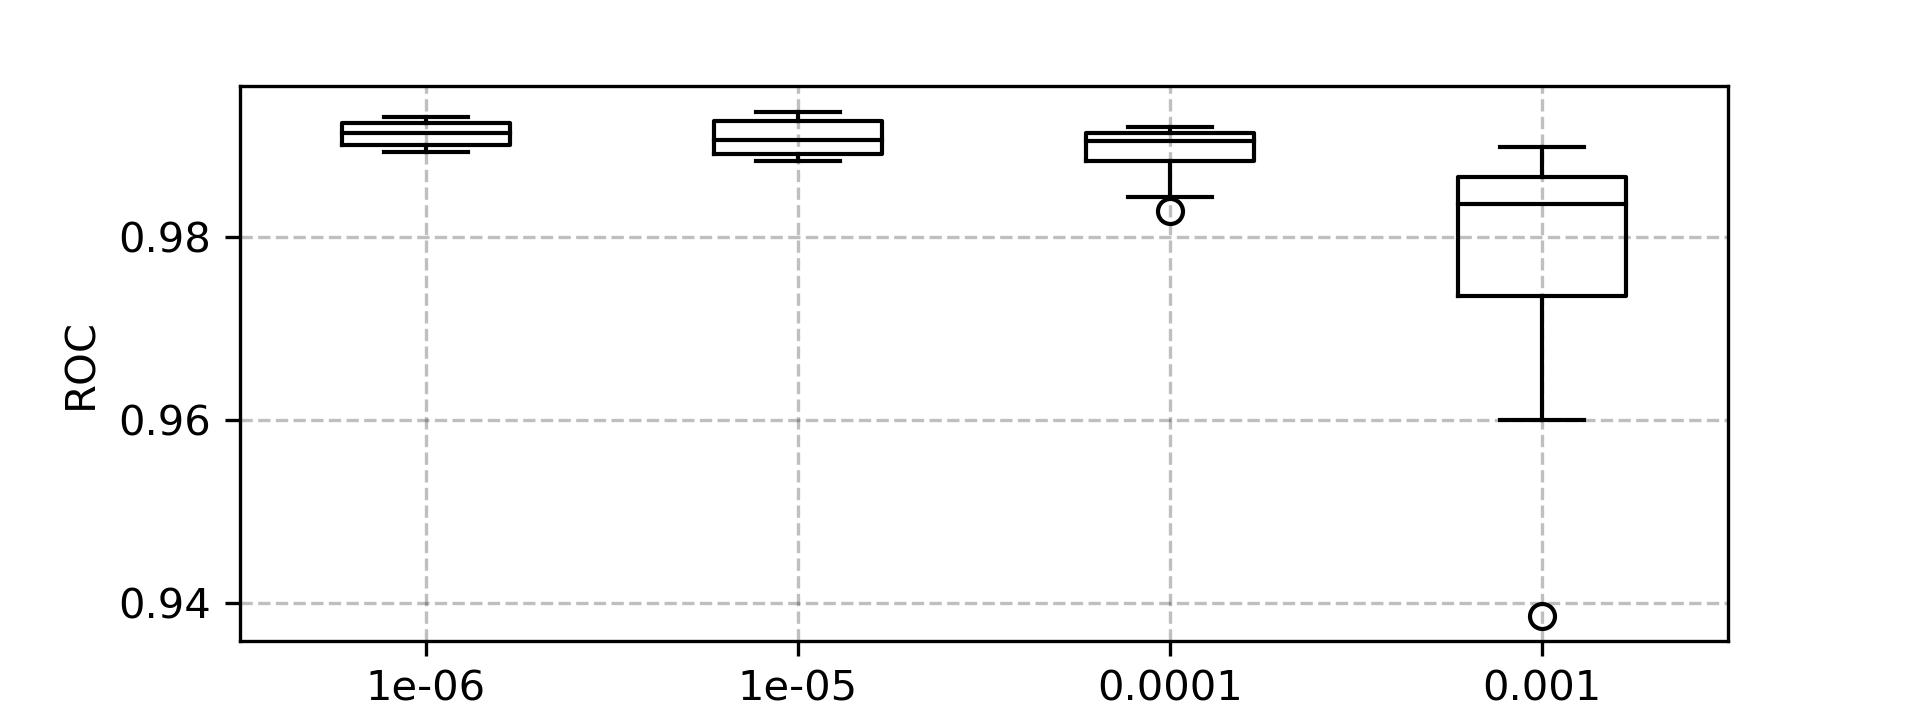
\includegraphics[width=\textwidth]{mtask/supp/densenet121_ulg_lbtd2_chimio_necrose_learning_rate.png}\\
    \caption{Necrose}
  \end{subfigure}
  \begin{subfigure}{0.48\textwidth}
    \centering
    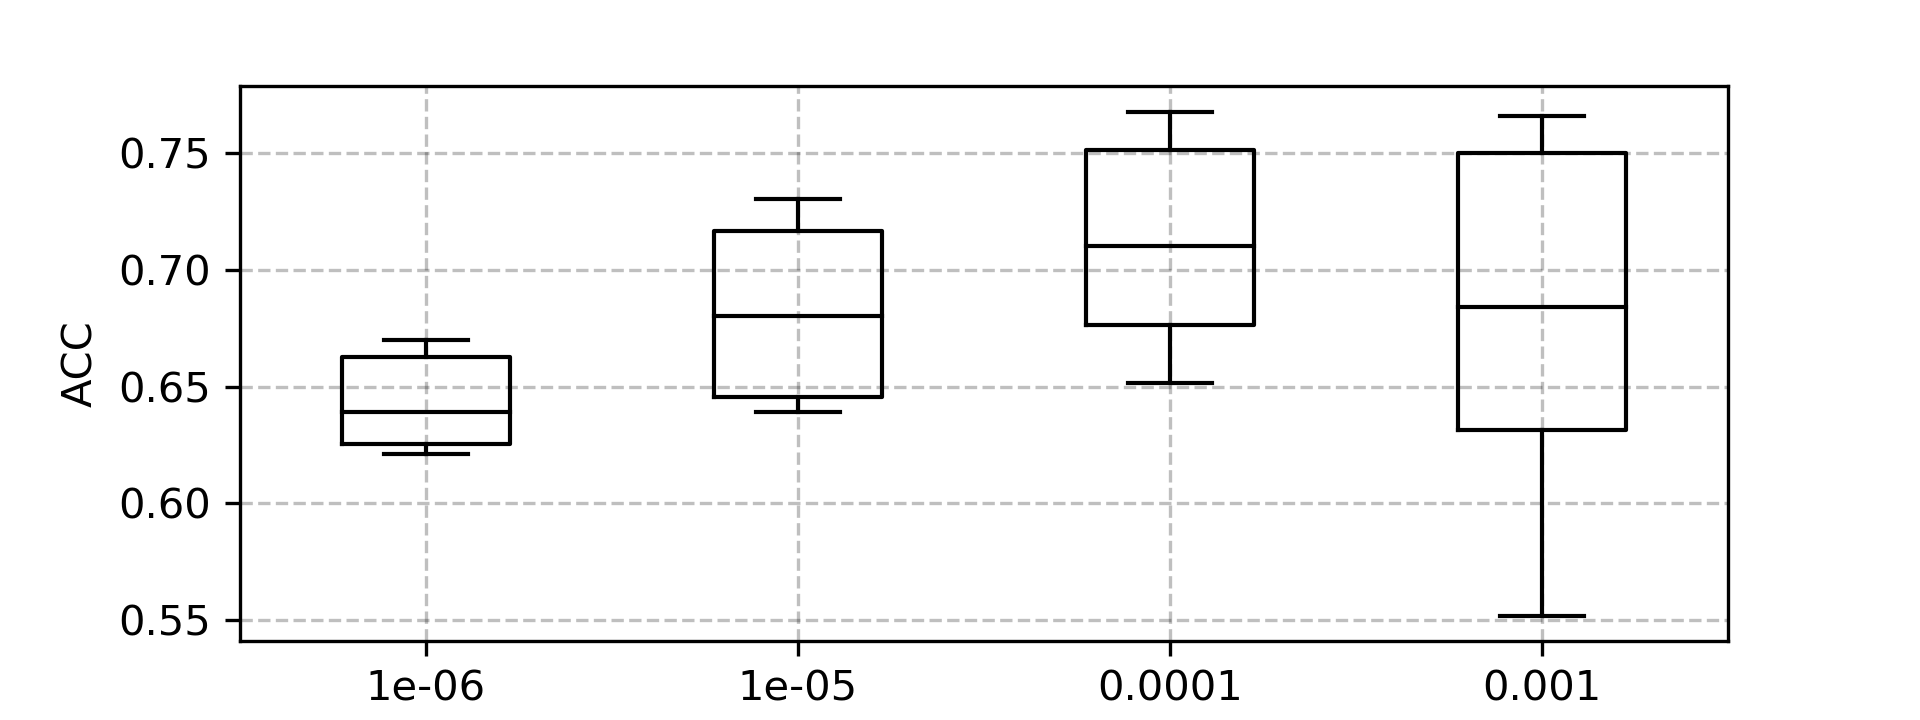
\includegraphics[width=\textwidth]{mtask/supp/densenet121_ulg_lbtd_lba_learning_rate.png}
    \caption{MouseLba}
  \end{subfigure}
  \begin{subfigure}{0.48\textwidth}
    \centering
    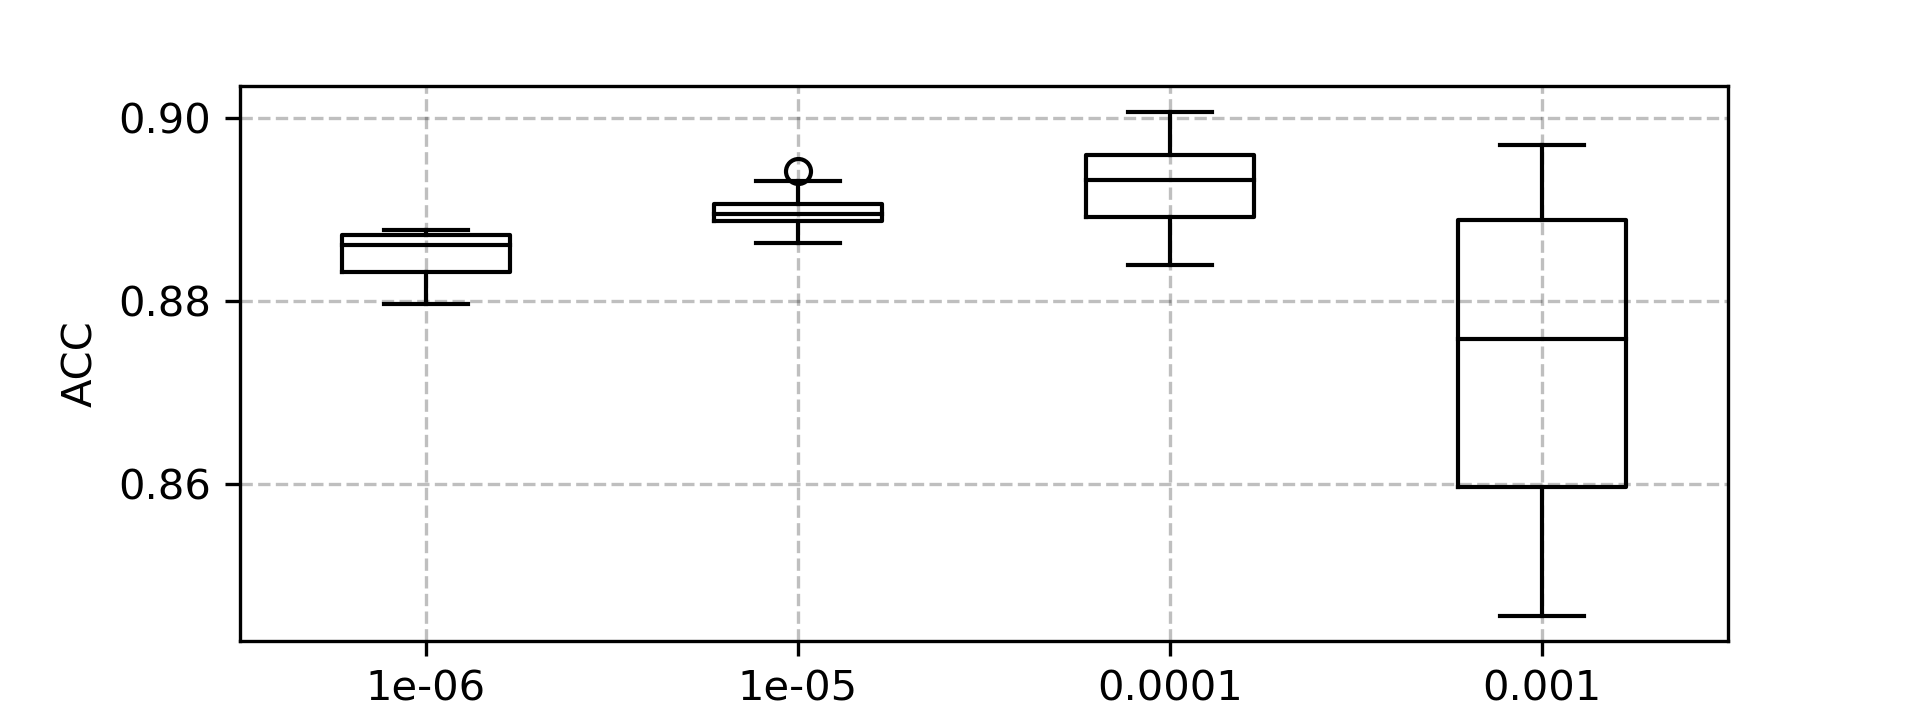
\includegraphics[width=\textwidth]{mtask/supp/densenet121_ulg_lbtd_tissus_learning_rate.png}
    \caption{Lung}
  \end{subfigure}
  \caption{Distributions of scores per learning rate on DenseNet121. Each boxplot results from the aggregation of the transfer scores of all models using the a learning rate value on the given network and dataset.}
  \label{app:mtask:fig:lr_densenet}
\end{figure*}

\begin{figure*}[h]
  \centering
  \begin{subfigure}{0.48\textwidth}
      \centering
      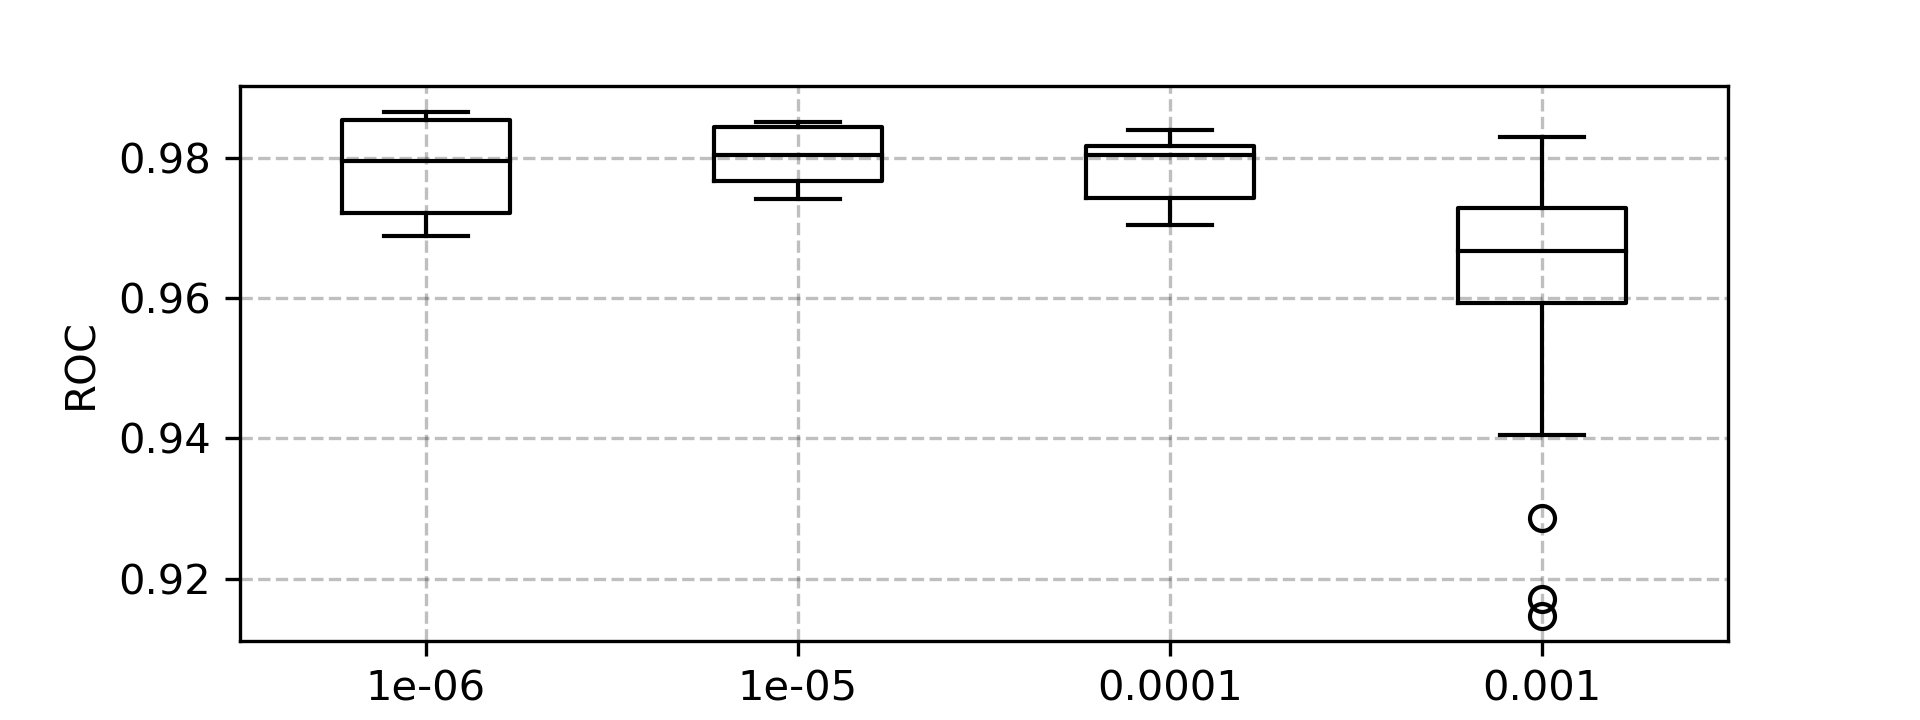
\includegraphics[width=\textwidth]{mtask/supp/resnet50_cells_no_aug_learning_rate.png}
    \caption{CellInclusion}
    \end{subfigure}
  \begin{subfigure}{0.48\textwidth}
    \centering
    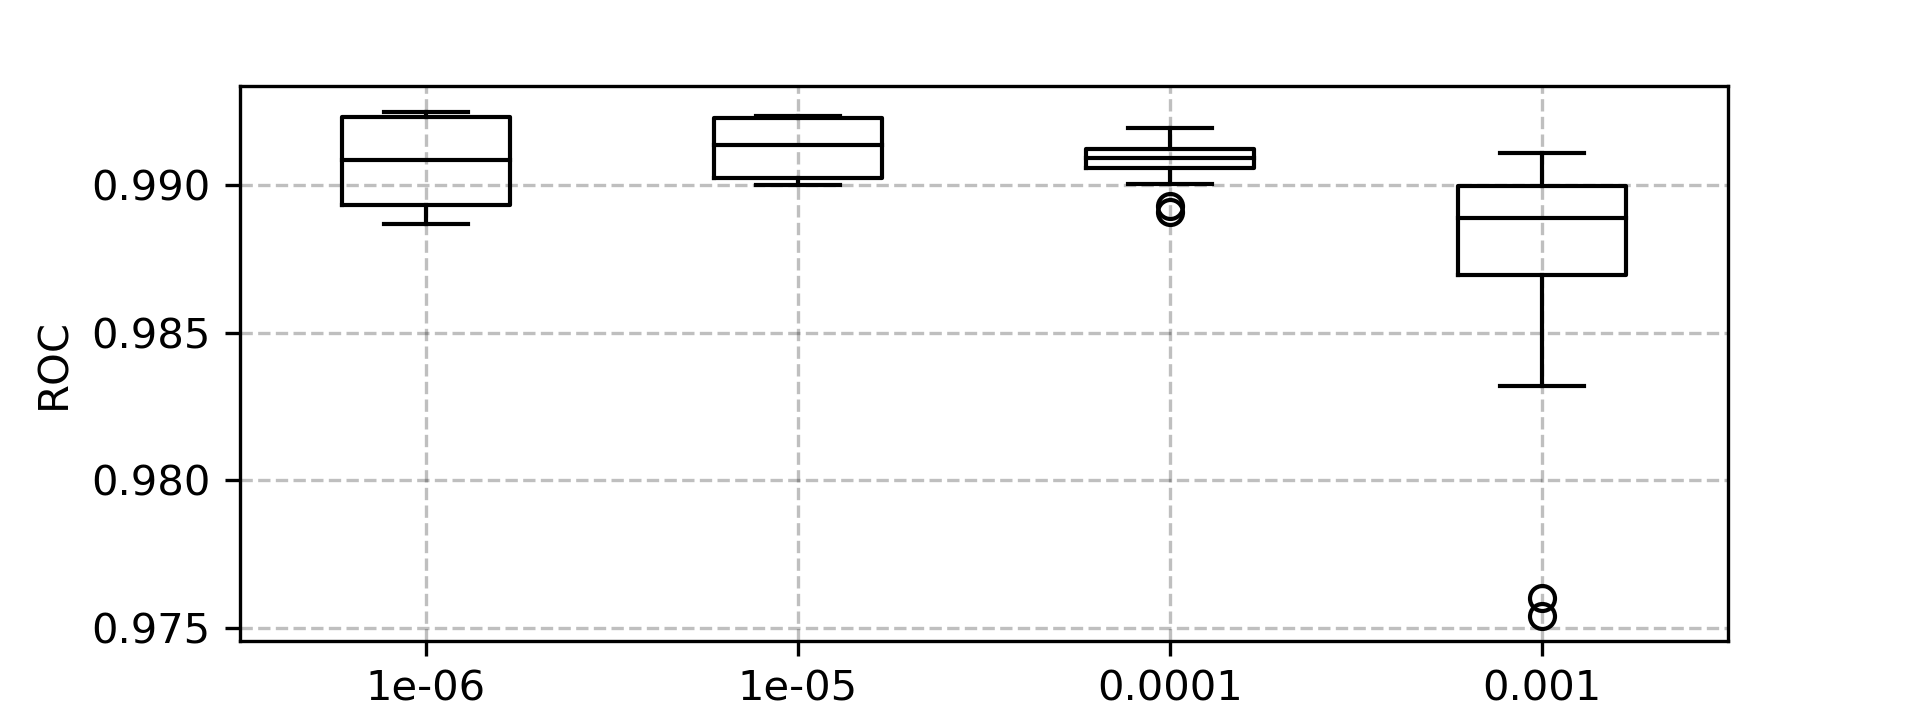
\includegraphics[width=\textwidth]{mtask/supp/resnet50_glomeruli_no_aug_learning_rate.png}\\
    \caption{Glomeruli}
  \end{subfigure}
  \begin{subfigure}{0.48\textwidth}
    \centering
    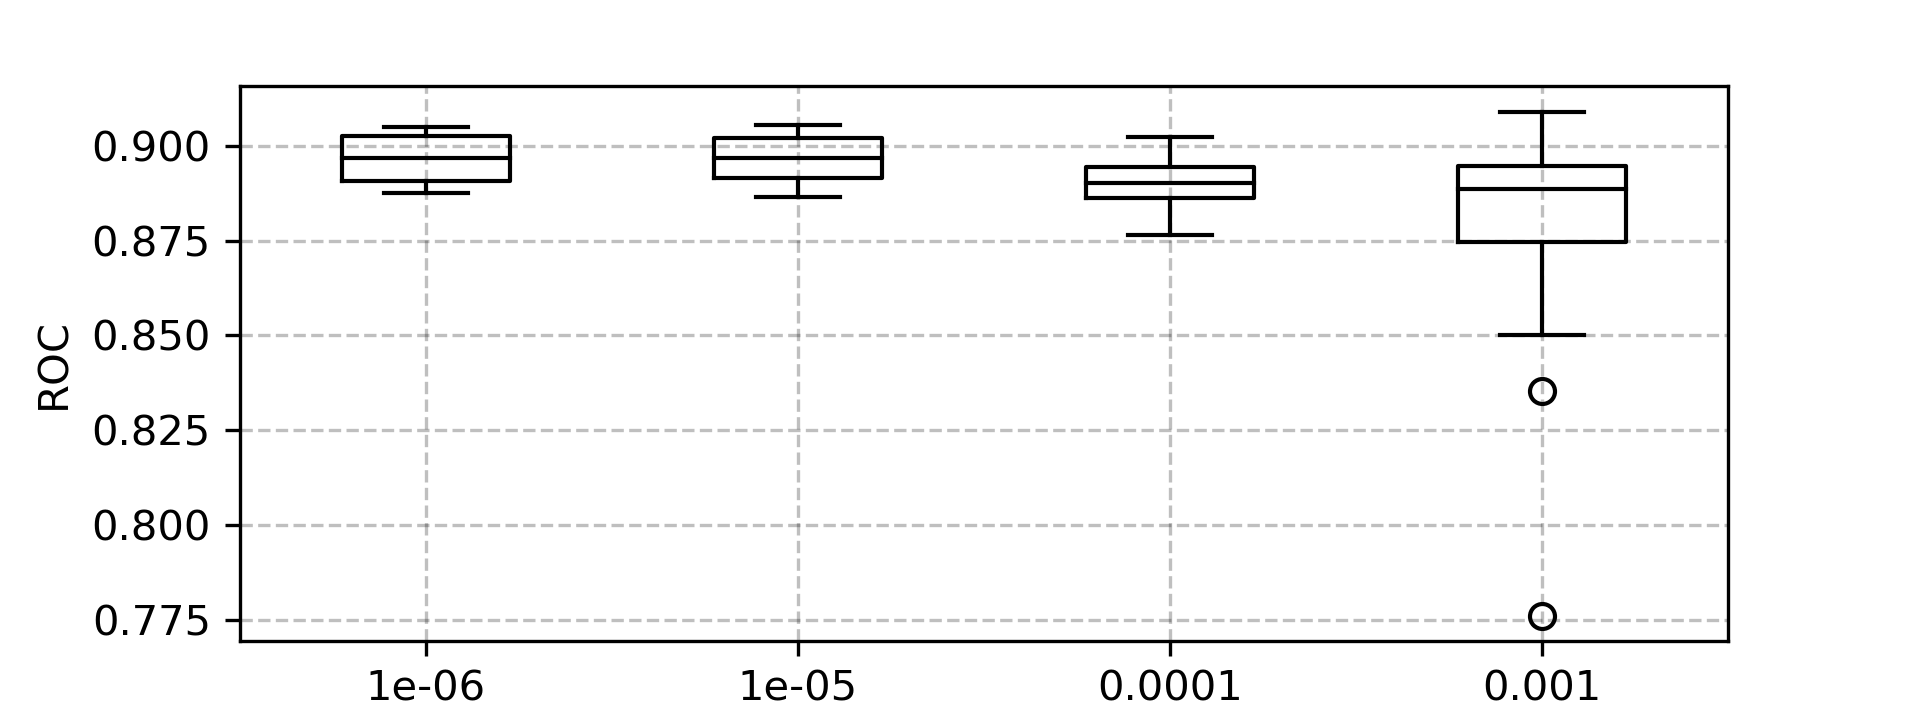
\includegraphics[width=\textwidth]{mtask/supp/resnet50_patterns_no_aug_learning_rate.png}
    \caption{ProliferativePattern}
  \end{subfigure}
  \begin{subfigure}{0.48\textwidth}
    \centering
    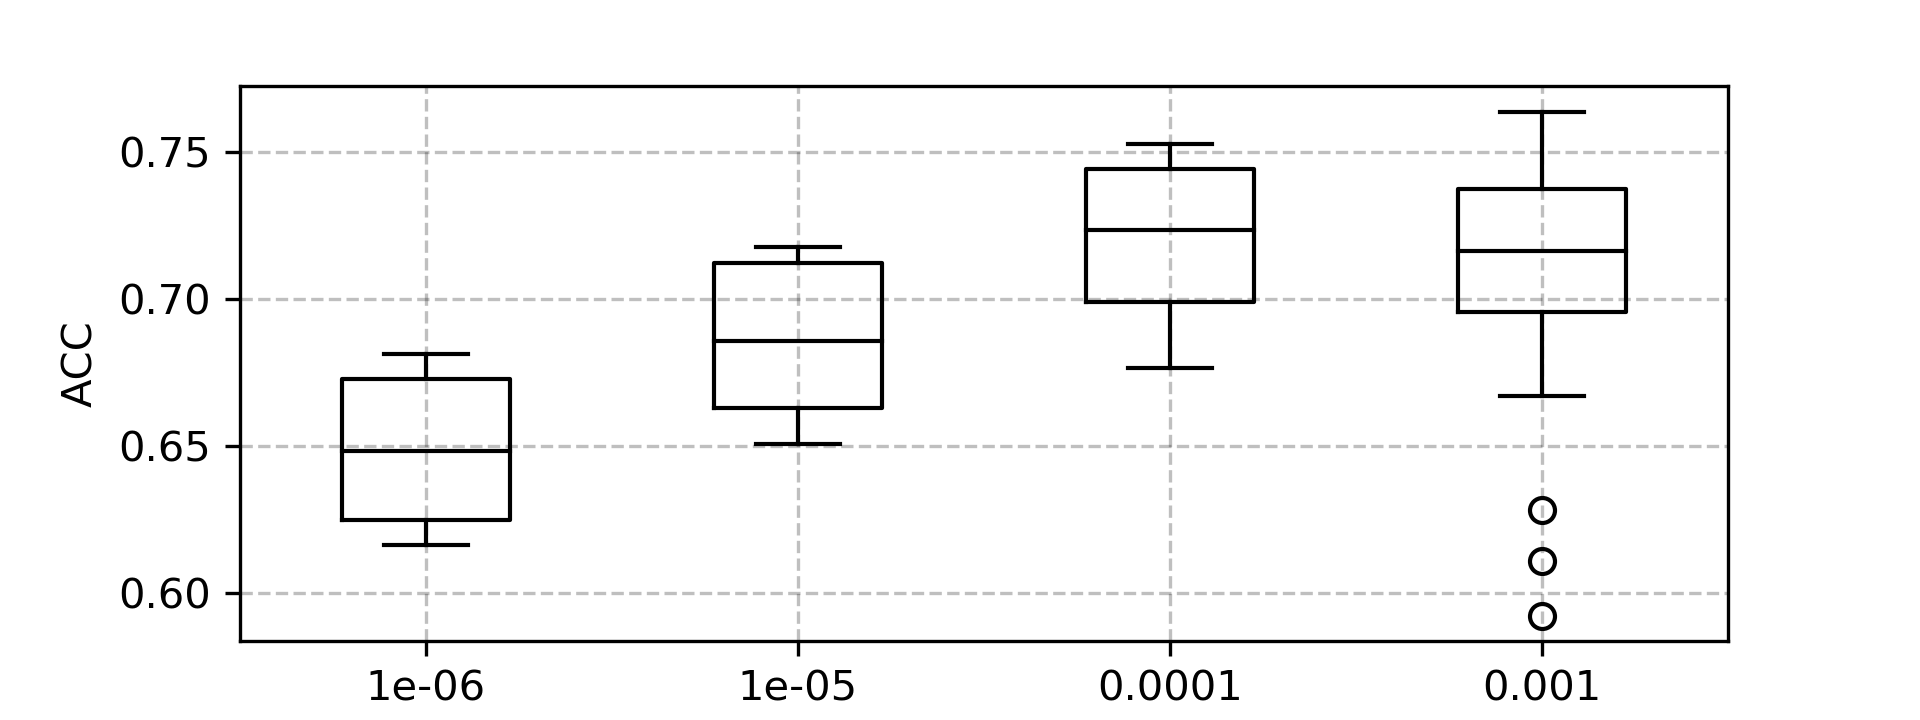
\includegraphics[width=\textwidth]{mtask/supp/resnet50_ulb_anapath_lba_learning_rate.png}\\
    \caption{HumanLba}
  \end{subfigure}
  \begin{subfigure}{0.48\textwidth}
    \centering
    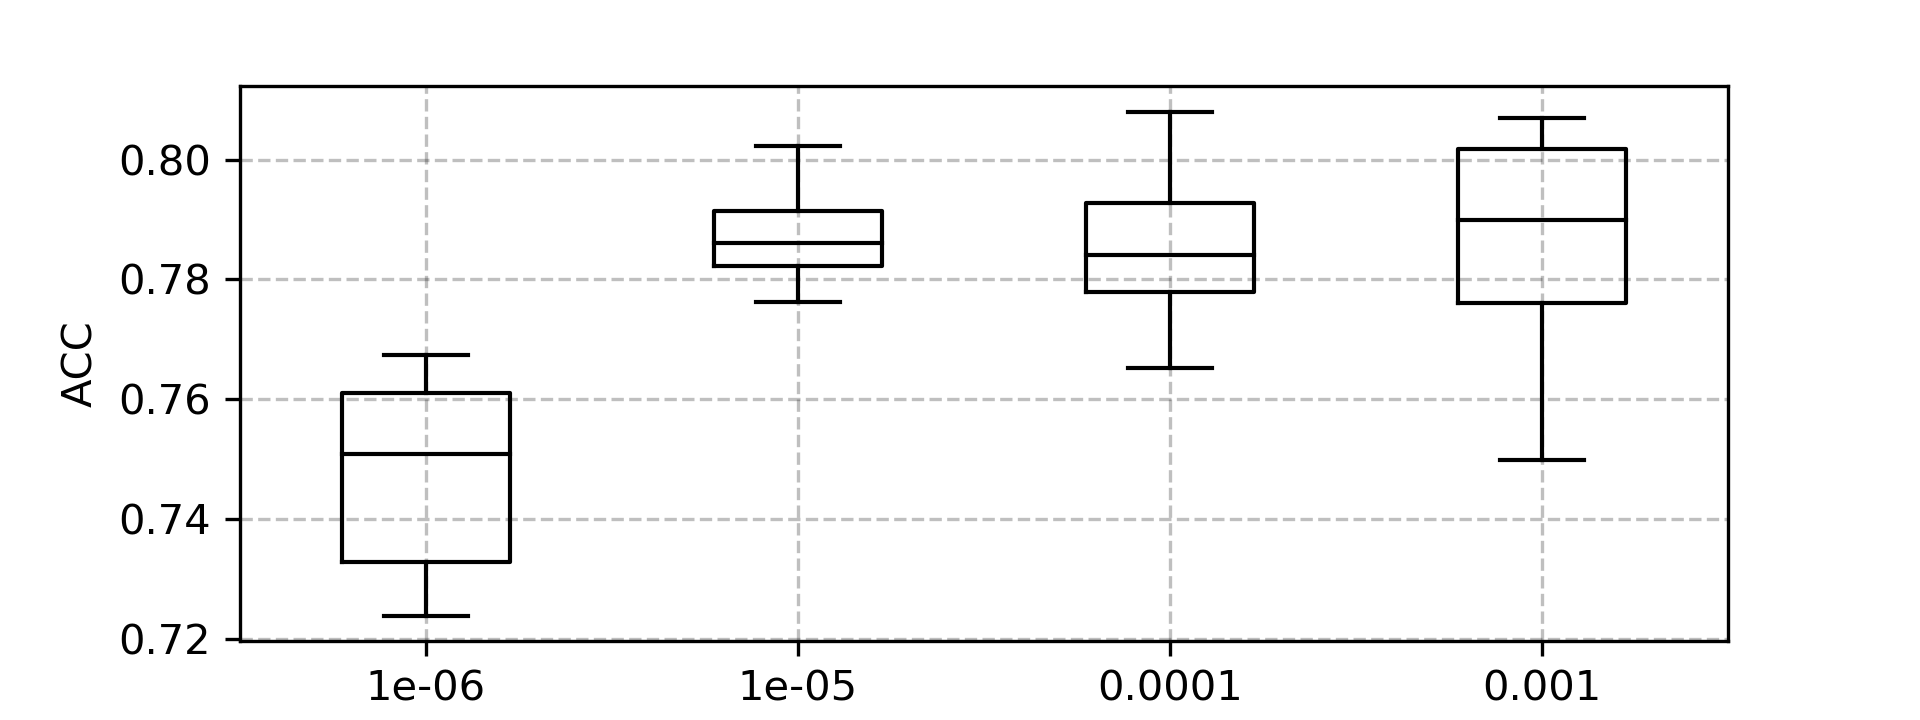
\includegraphics[width=\textwidth]{mtask/supp/resnet50_ulg_bonemarrow_learning_rate.png}
    \caption{BoneMarrow}
  \end{subfigure}
  \begin{subfigure}{0.48\textwidth}
    \centering
    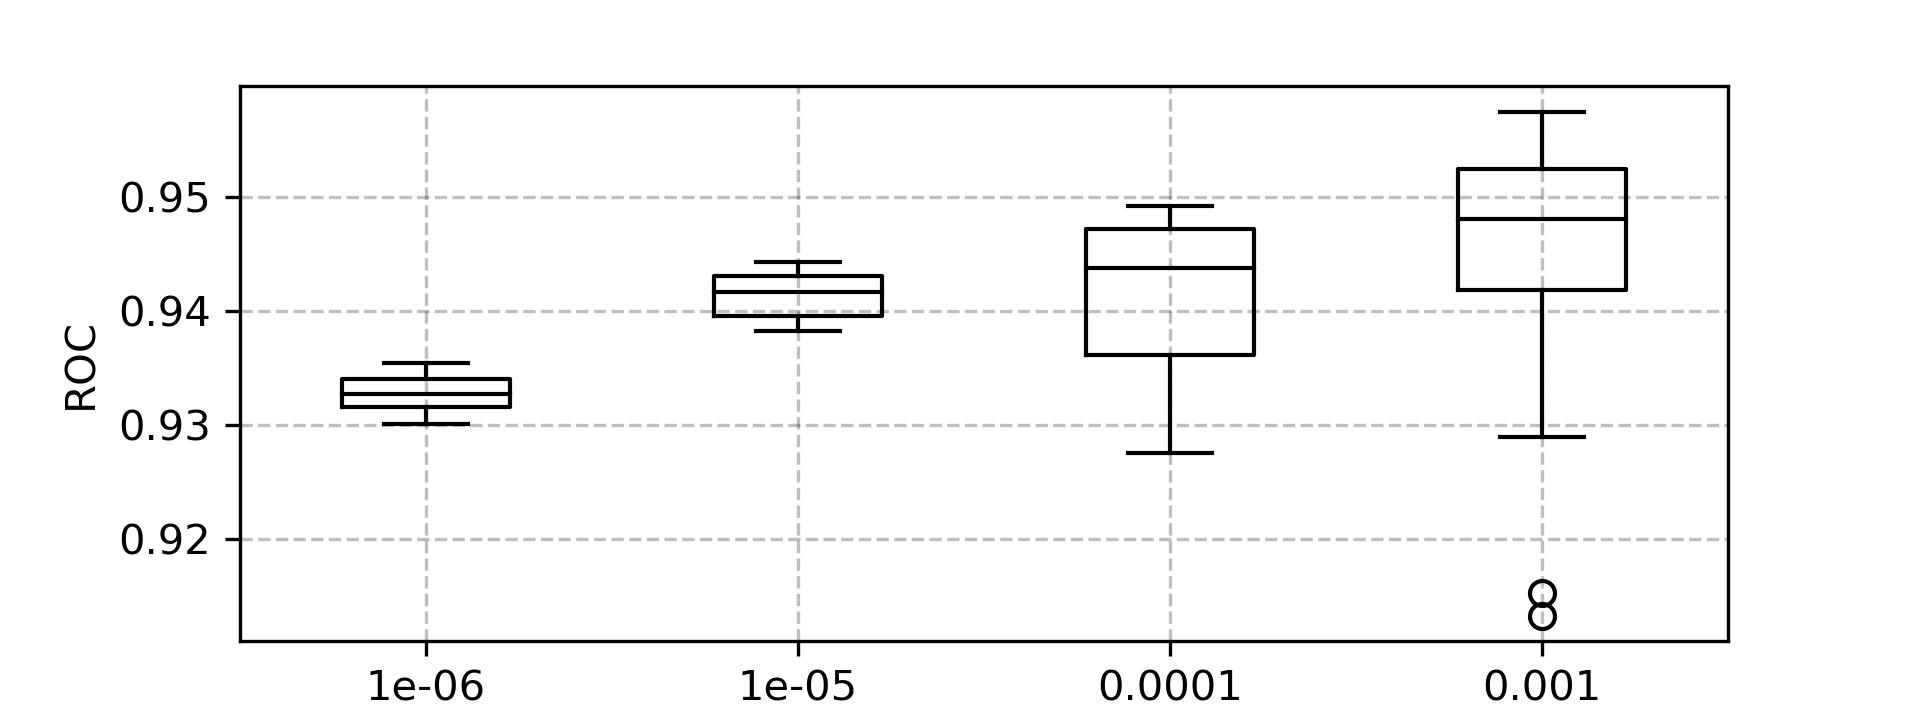
\includegraphics[width=\textwidth]{mtask/supp/resnet50_ulg_breast_learning_rate.png}\\
    \caption{Breast1}
  \end{subfigure}
  \begin{subfigure}{0.48\textwidth}
    \centering
    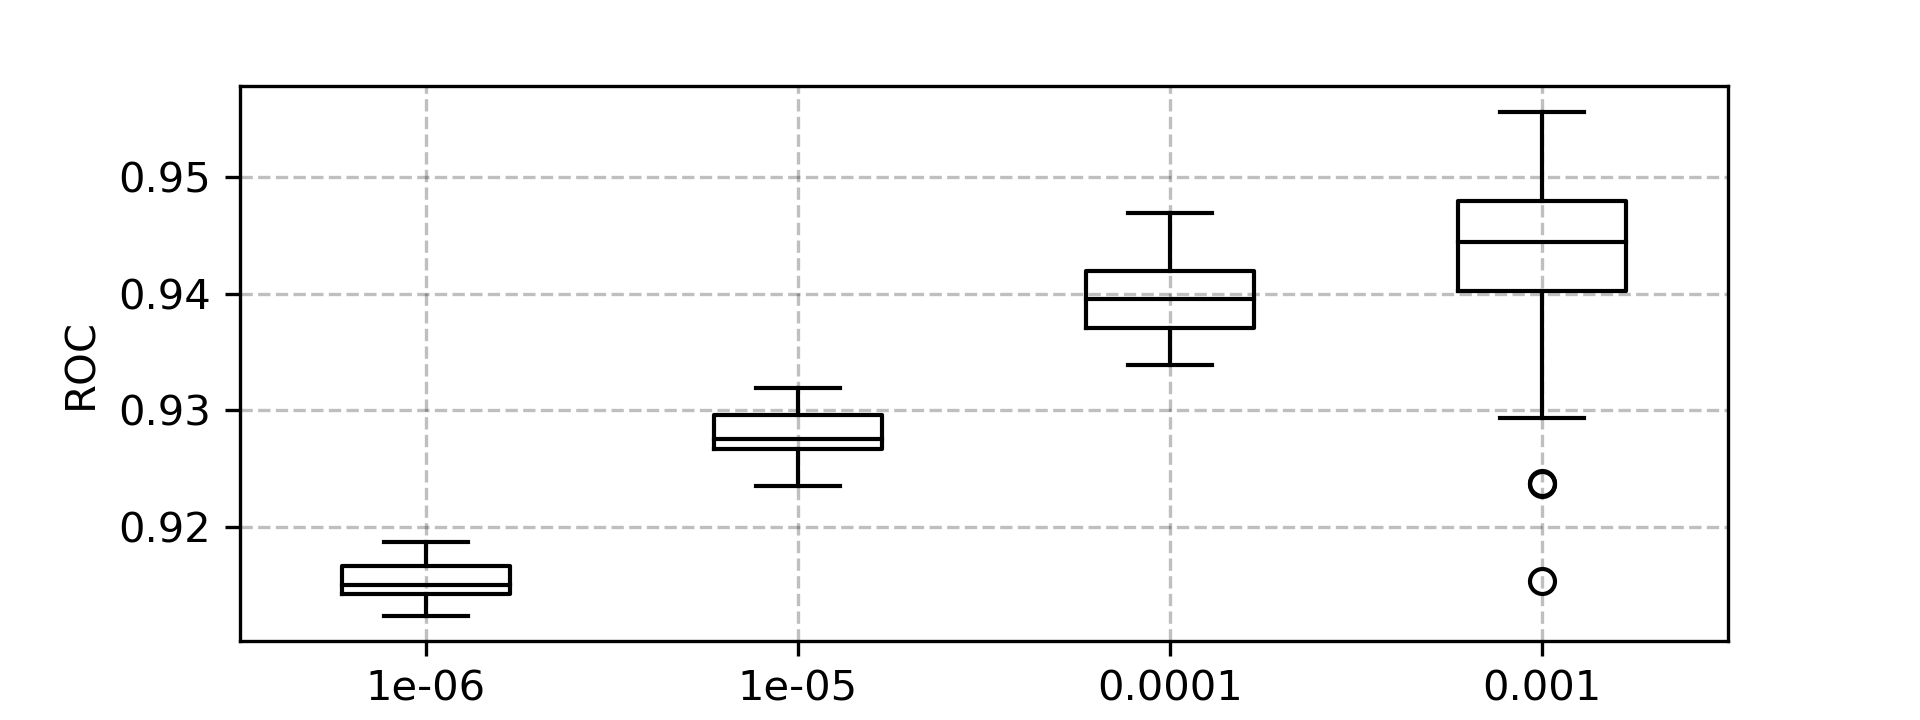
\includegraphics[width=\textwidth]{mtask/supp/resnet50_ulg_breast2_learning_rate.png}
    \caption{Breast2}
  \end{subfigure}
  \begin{subfigure}{0.48\textwidth}
    \centering
    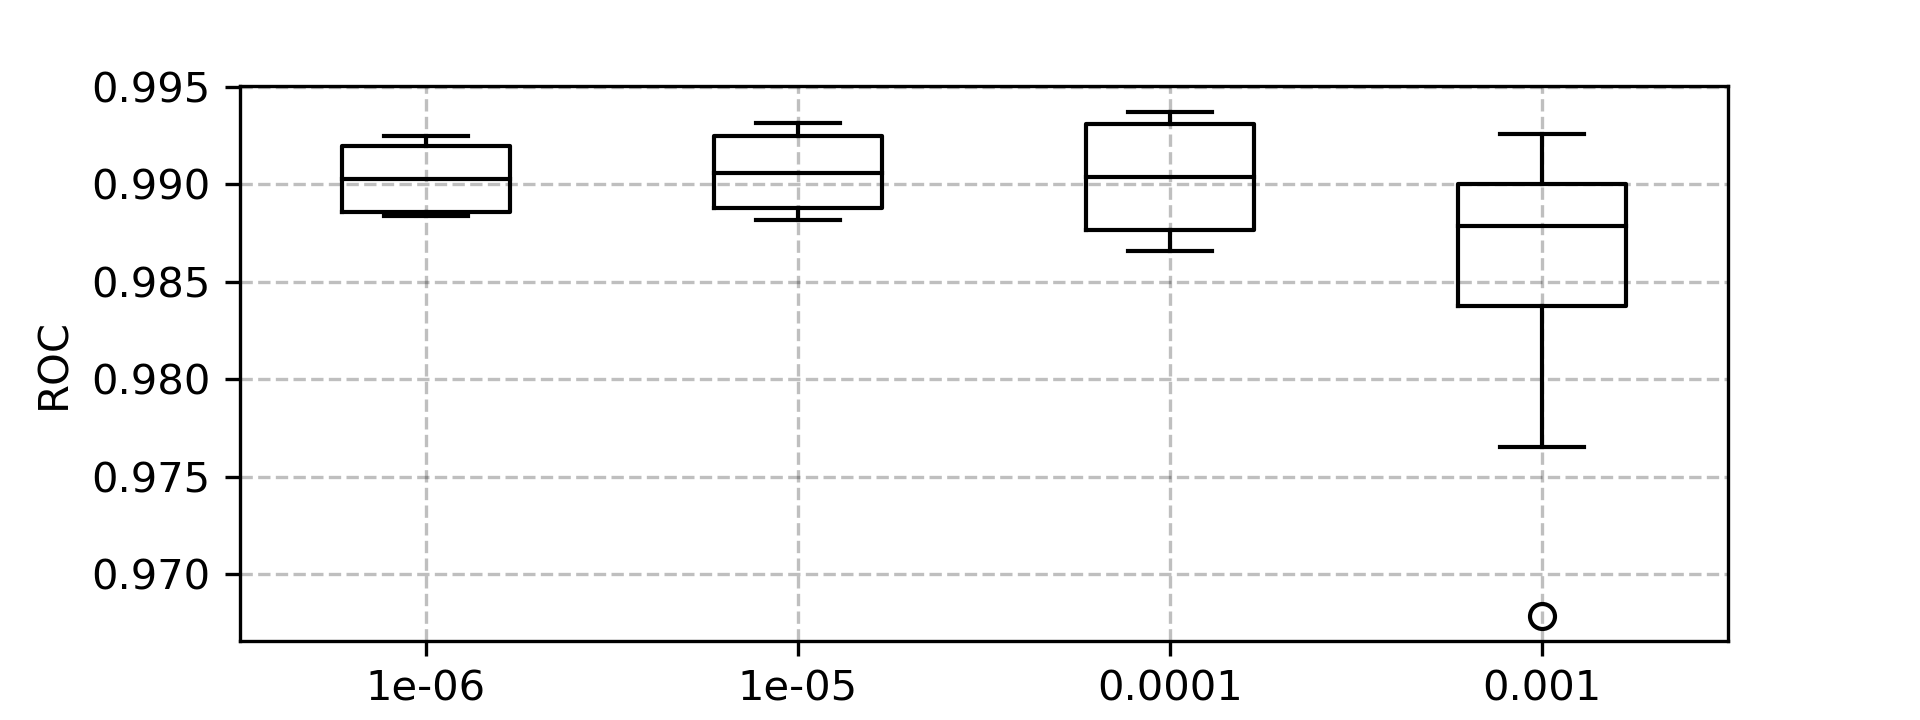
\includegraphics[width=\textwidth]{mtask/supp/resnet50_ulg_lbtd2_chimio_necrose_learning_rate.png}\\
    \caption{Necrose}
  \end{subfigure}
  \begin{subfigure}{0.48\textwidth}
    \centering
    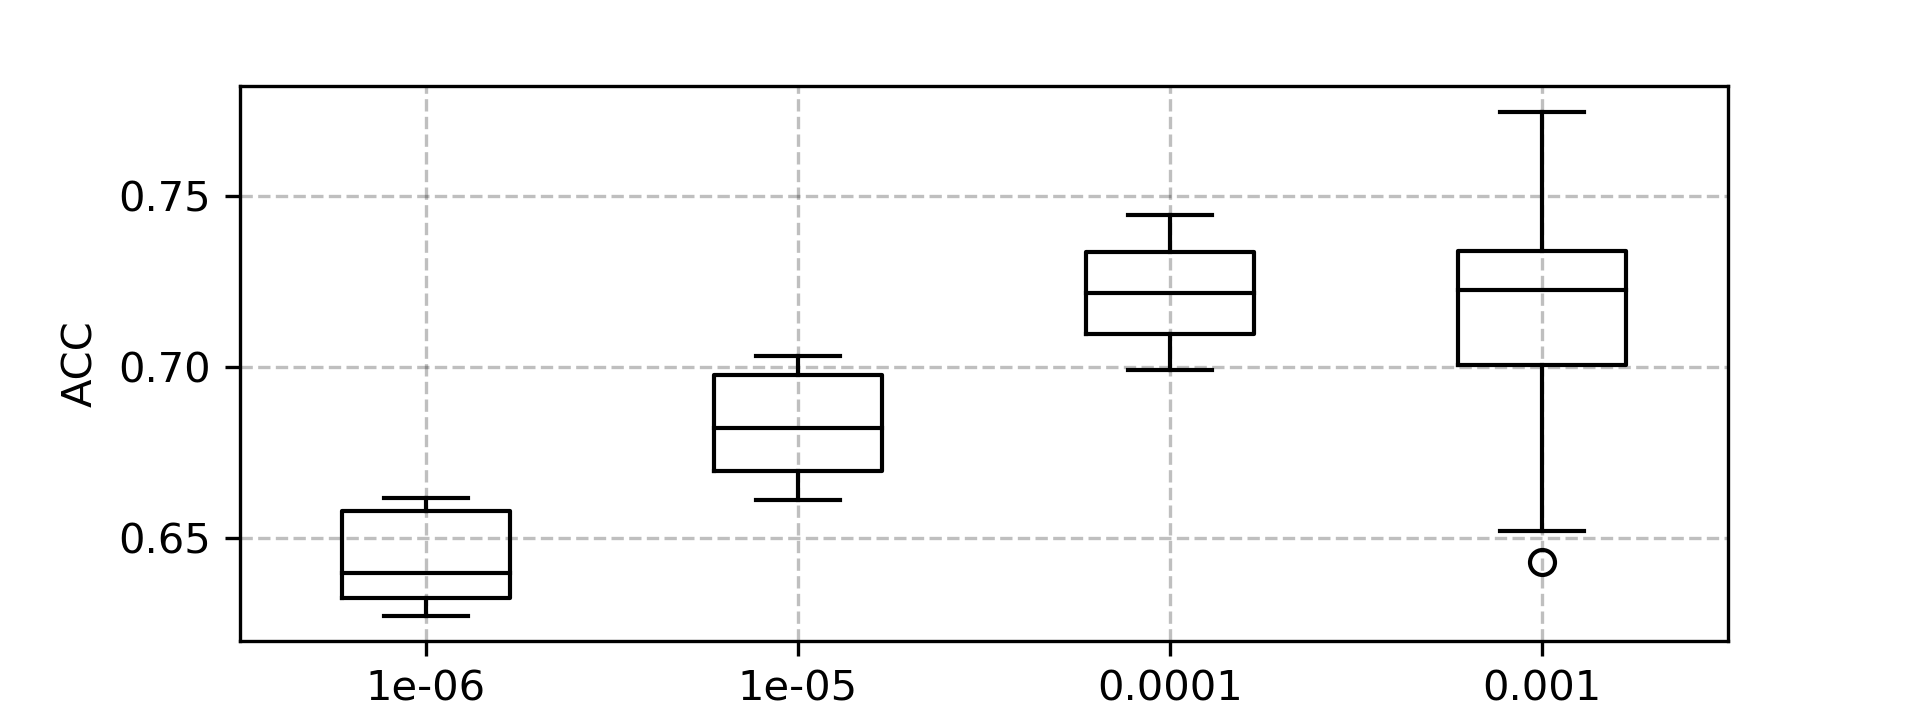
\includegraphics[width=\textwidth]{mtask/supp/resnet50_ulg_lbtd_lba_learning_rate.png}
    \caption{MouseLba}
  \end{subfigure}
  \begin{subfigure}{0.48\textwidth}
    \centering
    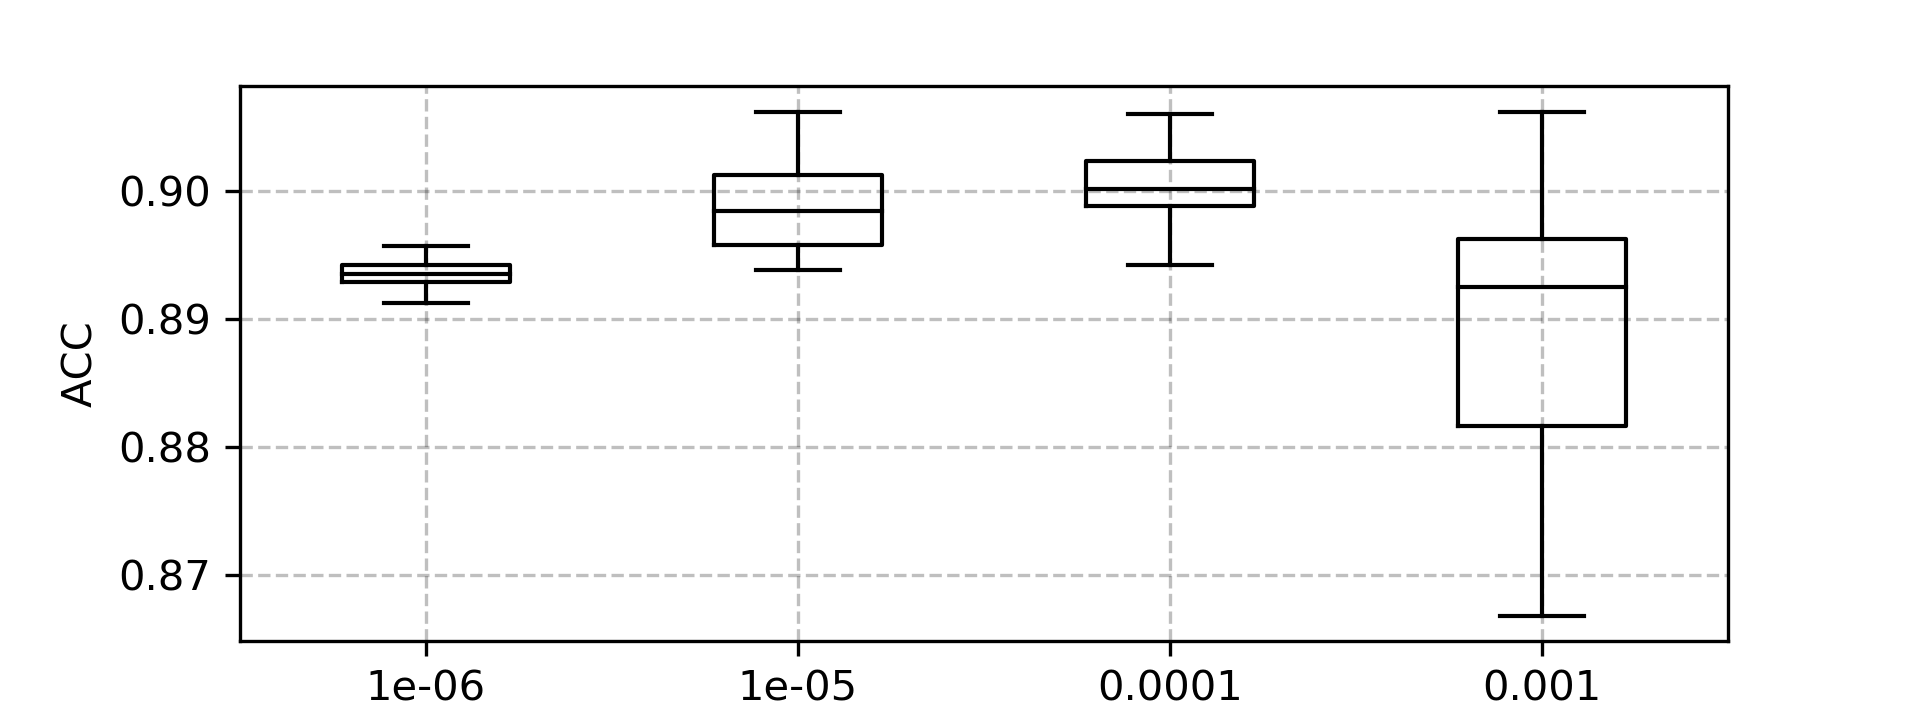
\includegraphics[width=\textwidth]{mtask/supp/resnet50_ulg_lbtd_tissus_learning_rate.png}
    \caption{Lung}
  \end{subfigure}
  \caption{Distributions of scores per learning rate on ResNet50. Each boxplot results from the aggregation of the transfer scores of all models using the a learning rate value on the given network and dataset.}
  \label{app:mtask:fig:lr_resnet}
\end{figure*}